%%%%%%%%%%%%%%%%%%%%%%%%%%%%%%%%%%%%%%%%%%%%%%%%%%%%%%%%%%%%%%%%%%%%%%
%%  disstemplate.tex, to be compiled with latex.		     %
%%  22 Feb 2019 	Version 5				     %
%%%%%%%%%%%%%%%%%%%%%%%%%%%%%%%%%%%%%%%%%%%%%%%%%%%%%%%%%%%%%%%%%%%%%%
%%								     %
%%  Writing a Doctoral Dissertation with LaTeX at		     %
%%	the University of Texas at Austin			     %
%%								     %
%%  (Modify this ``template'' for your own dissertation.)	     %
%%								     %
%%%%%%%%%%%%%%%%%%%%%%%%%%%%%%%%%%%%%%%%%%%%%%%%%%%%%%%%%%%%%%%%%%%%%%


\documentclass[12pt]{report}	% The documentclass must be ``report''.

\usepackage[T1]{fontenc}

\usepackage{../utdiss3}  		% Dissertation package style file.

\emergencystretch=1em



%%%%%%%%%%%%%%%%%%%%%%%%%%%%%%%%%%%%%%%%%%%%%%%%%%%%%%%%%%%%%%%%%%%%%%
% Optional packages used for this sample dissertation. If you don't  %
% need a capability in your dissertation, feel free to comment out   %
% the package usage command.					     %
%%%%%%%%%%%%%%%%%%%%%%%%%%%%%%%%%%%%%%%%%%%%%%%%%%%%%%%%%%%%%%%%%%%%%%

\usepackage{amsmath,amsthm,amsfonts,amscd} 
				% Some packages to write mathematics.
\usepackage{eucal} 	 	% Euler fonts
\usepackage{verbatim}      	% Allows quoting source with commands.
\usepackage{makeidx}       	% Package to make an index.
\usepackage{graphicx}           % Including graphics
\usepackage{cite}         	% 
\usepackage[hyphens]{url}		% Allows good typesetting of web URLs.
\usepackage{draftcopy}		% Uncomment this line to have the
				% word, "DRAFT," as a background
				% "watermark" on all of the pages of
				% of your draft versions. When ready
				% to generate your final copy, re-comment
				% it out with a percent sign to remove
				% the word draft before you re-run
				% Makediss for the last time.

\graphicspath{{figs/}}          % place figs in separate directory

\author{Steve Han}  	% Required

\title{Demonstrations for Robots in Immersive Virtual Reality}
%\title{Towards Large-scale Humanoid Demonstration Data Collection Using VR Headsets}
                                                    % Required

%%%%%%%%%%%%%%%%%%%%%%%%%%%%%%%%%%%%%%%%%%%%%%%%%%%%%%%%%%%%%%%%%%%%%%
% NOTICE: The total number of supervisors and other members %%%%%%%%%%
%%%%%%%%%%%%%%% MUST be seven (7) or less! If you put in more, %%%%%%%
%%%%%%%%%%%%%%% they are put on the page after the Committee %%%%%%%%%
%%%%%%%%%%%%%%% Certification of Approved Version page. %%%%%%%%%%%%%%
%%%%%%%%%%%%%%%%%%%%%%%%%%%%%%%%%%%%%%%%%%%%%%%%%%%%%%%%%%%%%%%%%%%%%%

%%%%%%%%%%%%%%%%%%%%%%%%%%%%%%%%%%%%%%%%%%%%%%%%%%%%%%%%%%%%%%%%%%%%%%
%
% Enter names of the supervisor and co-supervisor(s), if any,
% of your dissertation committee. Put one name per line with
% the name in square brackets. The name on the last line, however,
% must be in curly braces.
%
% If you have only one supervisor, the entry below will read:
%
%	\supervisor
%		{Supervisor's Name}
%
% NOTE: Maximum three supervisors. Minimum one supervisor.
% NOTE: The Office of Graduate Studies will accept only two supervisors!
% 
%
\supervisor
	{Yuke Zhu}

%%%%%%%%%%%%%%%%%%%%%%%%%%%%%%%%%%%%%%%%%%%%%%%%%%%%%%%%%%%%%%%%%%%%%%
%
% Enter names of the other (non-supervisor) members(s) of your
% dissertation committee. Put one name per line with the name
% in square brackets. The name on the last line, however, must
% be in curly braces.
%
% NOTE: Maximum six other members. Minimum zero other members.
% NOTE: The Office of Graduate Studies may restrict you to a total
%	of six committee members.
%
%
\committeemembers
	{Etienne Vouga}

%%%%%%%%%%%%%%%%%%%%%%%%%%%%%%%%%%%%%%%%%%%%%%%%%%%%%%%%%%%%%%%%%%%%%%

%\previousdegrees{B.S.}
     % The abbreviated form of your previous degree(s).
     % E.g., \previousdegrees{B.S., MBA}.

%\graduationmonth{...}      
     % Graduation month, either May, August, or December, in the form
     % as `\graduationmonth{May}'. Do not abbreviate.
     %
     % The default value (either May, August, or December) is guessed
     % according to the time of running LaTeX.

%\graduationyear{...}   
     % Graduation year, in the form as `\graduationyear{2001}'.
     % Use a 4 digit (not a 2 digit) number.
     %
     % The default value is guessed according to the time of 
     % running LaTeX.

%\typist{...}       
     % The name(s) of typist(s), put `the author' if you do it yourself.
     % E.g., `\typist{Maryann Hersey and the author}'.
     %
     % The default value is `the author'.


%%%%%%%%%%%%%%%%%%%%%%%%%%%%%%%%%%%%%%%%%%%%%%%%%%%%%%%%%%%%%%%%%%%%%%
% Commands for master's theses and reports.			     %
%%%%%%%%%%%%%%%%%%%%%%%%%%%%%%%%%%%%%%%%%%%%%%%%%%%%%%%%%%%%%%%%%%%%%%
%
% If the degree you're seeking is NOT Doctor of Philosophy, uncomment
% (remove the % in front of) the following two command lines (the ones
% that have the \ as their second character).
%
\degree{MASTER OF SCIENCE IN COMPUTER SCIENCE}
\degreeabbr{MSCompSci}

% Uncomment the line below that corresponds to the type of master's
% document you are writing.
%
%\masterreport
\masterthesis


%%%%%%%%%%%%%%%%%%%%%%%%%%%%%%%%%%%%%%%%%%%%%%%%%%%%%%%%%%%%%%%%%%%%%%
% Some optional commands to change the document's defaults.	     %
%%%%%%%%%%%%%%%%%%%%%%%%%%%%%%%%%%%%%%%%%%%%%%%%%%%%%%%%%%%%%%%%%%%%%%
%
%\singlespacing
%\oneandonehalfspacing

%\singlespacequote
\oneandonehalfspacequote

\topmargin 0.125in	% Adjust this value if the PostScript file output
			% of your dissertation has incorrect top and 
			% bottom margins. Print a copy of at least one
			% full page of your dissertation (not the first
			% page of a chapter) and measure the top and
			% bottom margins with a ruler. You must have
			% a top margin of 1.5" and a bottom margin of
			% at least 1.25". The page numbers must be at
			% least 1.00" from the bottom of the page.
			% If the margins are not correct, adjust this
			% value accordingly and re-compile and print again.
			%
			% The default value is 0.125"

		% If you want to adjust other margins, they are in the
		% utdiss2-nn.sty file near the top. If you are using
		% the shell script Makediss on a Unix/Linux system, make
		% your changes in the utdiss2-nn.sty file instead of
		% utdiss2.sty because Makediss will overwrite any changes
		% made to utdiss2.sty.

%%%%%%%%%%%%%%%%%%%%%%%%%%%%%%%%%%%%%%%%%%%%%%%%%%%%%%%%%%%%%%%%%%%%%%
% Some optional commands to be tested.				     %
%%%%%%%%%%%%%%%%%%%%%%%%%%%%%%%%%%%%%%%%%%%%%%%%%%%%%%%%%%%%%%%%%%%%%%

% If there are 10 or more sections, 10 or more subsections for a section,
% etc., you need to make an adjustment to the Table of Contents with the
% command \longtocentry.
%
%\longtocentry 



%%%%%%%%%%%%%%%%%%%%%%%%%%%%%%%%%%%%%%%%%%%%%%%%%%%%%%%%%%%%%%%%%%%%%%
%	Some math support.					     %
%%%%%%%%%%%%%%%%%%%%%%%%%%%%%%%%%%%%%%%%%%%%%%%%%%%%%%%%%%%%%%%%%%%%%%
%
%	Theorem environments (these need the amsthm package)
%
%% \theoremstyle{plain} %% This is the default

\newtheorem{thm}{Theorem}[section]
\newtheorem{cor}[thm]{Corollary}
\newtheorem{lem}[thm]{Lemma}
\newtheorem{prop}[thm]{Proposition}
\newtheorem{ax}{Axiom}

\theoremstyle{definition}
\newtheorem{defn}{Definition}[section]

\theoremstyle{remark}
\newtheorem{rem}{Remark}[section]
\newtheorem*{notation}{Notation}

%\numberwithin{equation}{section}


%%%%%%%%%%%%%%%%%%%%%%%%%%%%%%%%%%%%%%%%%%%%%%%%%%%%%%%%%%%%%%%%%%%%%%
%	Macros.							     %
%%%%%%%%%%%%%%%%%%%%%%%%%%%%%%%%%%%%%%%%%%%%%%%%%%%%%%%%%%%%%%%%%%%%%%
%
%	Here some macros that are needed in this document:


\newcommand{\latexe}{{\LaTeX\kern.125em2%
                      \lower.5ex\hbox{$\varepsilon$}}}

\newcommand{\amslatex}{\AmS-\LaTeX{}}

\chardef\bslash=`\\	% \bslash makes a backslash (in tt fonts)
			%	p. 424, TeXbook

\newcommand{\cn}[1]{\texttt{\bslash #1}}

\makeatletter		% Starts section where @ is considered a letter
			% and thus may be used in commands.
\def\square{\RIfM@\bgroup\else$\bgroup\aftergroup$\fi
  \vcenter{\hrule\hbox{\vrule\@height.6em\kern.6em\vrule}%
                                              \hrule}\egroup}
\makeatother		% Ends sections where @ is considered a letter.
			% Now @ cannot be used in commands.

\makeindex    % Make the index

%%%%%%%%%%%%%%%%%%%%%%%%%%%%%%%%%%%%%%%%%%%%%%%%%%%%%%%%%%%%%%%%%%%%%%
%		The document starts here.			     %
%%%%%%%%%%%%%%%%%%%%%%%%%%%%%%%%%%%%%%%%%%%%%%%%%%%%%%%%%%%%%%%%%%%%%%

\begin{document}

%
% NOTE: In a doctoral dissertation, the Committee Certification page
%		(with signatures) is BEFORE the Title page.
%	In a masters thesis or report, the Signature page
%		(with signatures) is AFTER the Title page.
%
%	If you are writing a masters thesis or report, you MUST REVERSE
%	the order of the \commcertpage and \titlepage commands below.
%
\commcertpage           % Produces the Committee Certification
			%   of Approved Version page (doctoral)
			%   or Signature page (masters).
			%		20 Mar 2002	cwm

\titlepage              % Produces the title page.




\begin{acknowledgments}		% Optional
\index{Acknowledgments@\emph{Acknowledgments}}%

Thanks to Mingyo Seo and Yuke Zhu for the project idea. 
Thanks to Mingyo Seo for creating the simulation, training the baselines, and adapting the whole body control code.
Thanks to Kyutae Sim for helping with the data collection.
Thanks to Carlos Isaac Gonzalez and Seung Hyeon Bang for help with the real robot experiments.
\end{acknowledgments}


% The abstract is required. Note the use of ``utabstract'' instead of
% ``abstract''! This was necessary to fix a page numbering problem.
% The abstract heading is generated automatically.
% Do NOT use \begin{abstract} ... \end{abstract}.
%
\utabstract
\index{Abstract}%
\indent
Our world is designed by humans, for humans. This makes humanoid robots the perfect general-purpose platform to automate repetitive or dangerous tasks done by people. However, due to the complexity of humanoid robots and the shortage of demonstration data, research in robot learning for humanoids is scarce. To address these challenges, I present a VR interface named DRIVR (Demonstrations for Robots in Immersive Virtual Reality) for collecting human demonstrations for humanoid robots in both simulation and reality. The demonstrations are then used to train a baseline imitation learning algorithm that uses an underlying controller to abstract away the complexity of whole-body control. I further propose that by embedding this data collection mechanism in VR video games, we can amass a large-scale dataset of high quality human demonstrations that can drive the development of future autonomous humanoids. To illustrate the feasibility of this idea, I collect a small dataset on toy tasks in simulation and a real robot using the VR interface. I then show that the trained policy can be deployed with a reasonable success rate.


\tableofcontents   % Table of Contents will be automatically
                   % generated and placed here.

\listoftables      % List of Tables and List of Figures will be placed
\listoffigures     % here, if applicable.



%%%%%%%%%%%%%%%%%%%%%%%%%%%%%%%%%%%%%%%%%%%%%%%%%%%%%%%%%%%%%%%%%%%%%%
% Actual text starts here.					     %
%%%%%%%%%%%%%%%%%%%%%%%%%%%%%%%%%%%%%%%%%%%%%%%%%%%%%%%%%%%%%%%%%%%%%%
%
% Including external files for each chapter makes this document simpler,
% makes each chapter simpler, and allows for generating test documents
% with as few as zero chapters (by commenting out the include statements).
% This allows quicker processing by the Makediss command file in case you
% are not working on a specific, long and slow to compile chapter. You
% can even change the chapter order by merely interchanging the order
% of the include statements (something I found helpful in my own
% dissertation).
%
\chapter{Introduction}
\index{Introduction@\emph{Introduction}}%


This document deals with how to write a doctoral dissertation 
using \LaTeX{}, and how to use the \texttt{utdiss2} package. 
\index{utdiss2 package@{\texttt{utdiss2} package}}%

The latest version of this document/package can be obtained from
\url{http://www.ph.utexas.edu/~laser/craigs_stuff/LaTeX/}.\footnote{I
will be transferring this page to the Office of Graduate
Studies when I graduate. The new URL isn't defined yet, but I will
place a ``redirect'' at this URL to send your browser to the correct
location when the transition occurs.}
If your installation of LaTeX is missing any style files used in this
document (most likely with a \cn{usepackage\{package-name.sty\}}
command at the beginning of disstemplate.tex), take a look at the link
on this page to ``Frequently Requested Style Files'' or on the
Comprehensive TeX Archive Network, \url{http://www.ctan.org}.

In case of any confict between the requirements of the Office of Graduate
Studies and what this document says to do, the requirements of the Office
of Graduate Studies prevail.

\section{History of This Package}
\index{History of This Package@\emph{History of This Package}}%

In 1991 the \texttt{utdiss} package was written by Young U. Ryu 
\index{Young U. Ryu}%
in order to be used in the preamble of \LaTeX{} doctoral dissertation
files at the University of Texas at Austin. 
\index{University of Texas at Austin}%
Since then some changes have occured, the most important one
being the introduction of a new version of \LaTeX{} 
\index{LaTeX@{\LaTeX{}}}%
called \LaTeXe{}. 
\index{LaTeX2e@{\LaTeXe{}}}%

In order to partially adapt the utdiss package to this new version
of \LaTeX{}, Miguel Lerma introduced a few modifications in it,
and his document, \textit{How to Write a Doctoral Dissertation
with \LaTeX{}}, served as a test for it. His new package was
called \texttt{utdiss1}.
\index{utdiss1@\texttt{utdiss1}}%

With the significant changes in style introduced by the Graduate
School in the Spring of 2001, as well as  my need to write a
dissertation myself, I extended Miguel Lerma's package to meet
these new requirements. As in Miguel Lerma's case, this document
serves as a test for it, but it is, in addition, intended as a
template for others to use in writing their own dissertations.
The new package is called \texttt{utdiss2}.
\index{utdiss2@\texttt{utdiss2}}%

\section{Revised Philosophy for This Package}
\index{Revised Philosophy for This Package@\emph{Revised Philosophy
	for This Package}}%

Since the source file of this document is intended to be used by students
writing their own dissertations, this document does not display all of the
comments regarding usage of previous versions. It has, instead, transferred
these comments to their respective places in the source file so someone
editing their own copy of the source file to produce their own dissertation
will see the comments where they are needed. It may be helpful to print out
a copy of the source file along with the PostScript version of the document
so the two can be studied side-by-side.

\textbf{Note:} In spite of the effort to accommodate the package to
the requirements of the University, it is not possible to guarantee
that it will always work, and the author of the dissertation remains
responsible for checking that such requirements are actually fulfilled
by his/her final work. 

The standard caveat applies:

\begin{quote}
\index{guarantee}%
This template package is provided and licensed ``as is'' without warranty
of any kind, either expressed or implied, including, but not limited to,
the implied warranties of merchantability and fitness for a particular
purpose. Yadda, yadda, yadda, \ldots
\end{quote}

In case of any problem with the use of \texttt{utdiss2}, send me email
at \url{mccluskey@mail.utexas.edu}.

\chapter{Background}

In this chapter, the necessary background information for this work is introduced. Then, existing literature that relates to our goal will be surveyed.

\section{Imitation Learning}

In imitation learning, a task is demonstrated by a human instructor multiple times until a robot can imitate the demonstrated behavior and perform the task autonomously. 
There are many forms of imitation learning.
The simplest form is Behavioral Cloning, where the robot learns to imitate the motion without inferring the actual goal. This becomes a supervised learning problem with the inputs being the observations and the outputs being the actions taken. This simple method is often effective \cite{zhang2018deep}, but it is prone to covariant shift \cite{ross2011reduction}, in which the errors in actions accumulate and the state deviates from the ones shown in demonstration. 
Another class of algorithms is inverse reinforcement learning, in which the agent tries to reverse-engineer the reward function from the demonstrations. 
However, this is usually computationally expensive due to the requirement to run reinforcement learning as an inner-loop.

The specific imitation learning algorithm used in our work is Behaviorial Cloning with Recurrent Neural Networks (RNN) and Gaussian Mixture Models (GMM). RNN maintains information about the past and can be viewed as injecting the inductive bias of sequentiality. Namely, it preserves time translation invariance by using the same neural network weights at each time step \cite{battaglia2018relational}. GMM uses a mixture of Gaussians with different means to approximate a multimodal distribution, such as the multiple ways that a human may do a specific task.

\section{Whole-body Control}

Whole-body control is a robotics approach that aims to control the entire robot's body, including its arms, legs, torso, and head, to achieve a desired task.
The specific form we are using is called implicit hierarchical whole-body controller \cite{Ahn2021VersatileLP}, which uses an implicit hierarchy of tasks to allow for different prioritization of control depending on whether the robot is performing locomotion or manipulation. For example, we would like the robot to prioritize foot motion over hand motion when the robot is walking.

Whole-body control can be formulated as finding the optimal joint acceleration $\ddot{q}^*$ and contact forces $f_r^*$ to minimize a loss function: 
$$
\min_{\ddot{q}, f_r}
 \sum_{i=1}^{n} 
  w_i \|J_i\ddot{q} 
   +\dot{J}_i\dot{q}_m
   -\ddot{x}_i^d\|^2
  +w_{f_r} \| f_r^d - f_r\|^2
  +\lambda_q \|\ddot{q}\|^2
  +\lambda_{f_r} \|f_r\|^2
$$
subject to the constraints of robot dynamics, contact, maximum reaction force, joint position limit, and torque limit.
The first term in the loss function represents the task space error, or the deviation of the robot's end-effector position and orientation from the desired values. The second term represents the contact force error. The third term regularizes the joint acceleration to control the trade-off between task performance and joint motion smoothness. The fourth term regularizes the contact force to prevent damage to the robot or the environment.

\section{Related Work}

\subsection{VR for Imitation Learning}

The work that most closely relates to ours is \cite{zhang2018deep}, which also involves using a consumer VR headset to teleoperate a robot. They show that by using only half an hour of demonstrations collected in VR, an imitation learning algorithm can be trained to perform simple manipulation tasks such as grabbing a ball or pushing a block. 
However, their robot has a fixed base, so they can directly use their robot's built-in Jacobian-transpose based controller instead of a whole-body controller. 
Instead of streaming stereoscopic images to the headset, they use Unity to render the colorized point cloud from the robot's 3D camera to allow the user to look around freely in the VR world. 
They argue that since the robot's head has low degrees of freedom and moves slowly, controlling its movement using the headset's movement will cause motion sickness. 
Indeed, we are faced with the same problem. 
However, instead of using a point cloud that could look strange for the demonstrator, we simply disallowed movements of the head.
This is sufficient for our tasks, and it does not seem to impact immersion. 
For learning, they also use a Behavior Cloning algorithm. 
However, they are only controlling one arm of the robot, whereas we are controlling both. 
They are also using the depth image as an input, but we only provide stereoscopic images. 
Finally, we are using an RNN to preserve information from previous time steps, while they only provide the 5 most recent end effector poses and no image history. 

Another work that utilizes VR for robot learning is \cite{arunachalam2022holodex}, which uses the hand-tracking capabilities of the Oculus Quest II headset to teach a robot hand dexterous manipulation skills. They first retarget the human hand joints to a robot hand with 4 fingers, then they use visual self-supervised learning combined with a simple nearest neighbor algorithm to successfully manipulate objects unseen during training. Although they are using a VR headset, they are not using stereoscopic rendering to create depth perception. Instead, they are rendering the robot's camera as a 2D video in Unity. Similarly, there is a senior thesis project teleoperating a small car in VR, and they also use a 2D video displayed through Unity \cite{carvr}. 

\subsection{Demonstration Interface}

There are multiple ways to collect demonstrations for imitation learning in existing literature. First, a teleoperation input device with 6 degrees of freedom such as the SpaceMouse can be used to control the position and orientation of the robot's end effector \cite{zhu2022robosuite}. However, it can be unintuitive for people to translate a 3D motion into the push and turn of a button, especially if there is a need to control 2 arms at once. In addition, since SpaceMouse controls the velocity instead of position, it requires training to perform actions involving precision. 
Second, humans can directly hold the robot to move it in a desired trajectory by applying force \cite{Akgn2012KeyframebasedLF} \cite{Schulman2013LearningFD}. This is called kinesthetic teaching, but it requires the human to come into the frame to control the robot, which becomes a problem when the policy is trained on vision data. To avoid this, we can also build a replica of the robot and move the replica manually, while the main robot follows its trajectory. For example, \cite{aloha} used a low-cost replica of their bi-manipulation robot to collect demonstrations for fine manipulation tasks. To do so, a human demonstrator pushes the end-effectors of the replica robot to backdrive its joints, and the resulting joint positions are issued as commands for the actual robot to follow. While this method achieved impressive results for the fixed-base robot, they cannot handle the floating-base dynamics of humanoid platforms, which requires torque control to account for the dynamics of the robot. 

Since we can manipulate a replica of the robot to create demonstrations, why can't we use our own body as this replica? After all, humanoids are design to mimic the morphology of humans. 
Indeed, we can directly record the kinematics of human motions \cite{Billard:2013}. Using either a camera or a motion capture system, we can measure the angular displacement of the joints precisely, and then we can map the values to the robot's joints. However, robots can have different mass distributions and degrees of freedom than humans. So, the actions that humans perform may be impossible for robots or cause them to lose balance. Therefore, learning a good mapping and using a whole-body controller to maintain balance are crucial to the success of this method.

\subsection{Learning for Humanoids}
As mentioned in the introduction, there does not seem to be prior work on training humanoid robots to perform manipulation tasks. 
Two works that cut close are \cite{4115578}, which uses Hidden Markov models to imitate a human demonstration, and \cite{7989550}, which uses motion planning to produce fluid transitions between locomotion, loco-manipulation, and manipulation. However, both works only consider a simple simulation with only kinematics and no dynamics, so their results are impossible to be applied to the real world.

Nonetheless, there are recent successes on learning humanoid locomotion.
\cite{kumar2022adapting} adapts the Rapid Motor Adaptation work \cite{kumar2021rma} to bipedal robots. It uses an adaptation module to enable the walking controller to adapt to changing environment in real-time. \cite{radosavovic2023learning} uses IsaacGym simulation to train a humanoid locomotion controller that responds to velocity commands robustly. Their work seems to be a more robust version of \cite{kumar2022adapting} where instead of explicitly adapting to the environment, the transformer implicitly infers the environment through past actions rapidly in every time step. Indeed, they showed that their controller can even maintain balance when objects are thrown at it. There have been attempts at using Isaac Gym and RL to train humanoids to walk in simulation in a brute-force manner without success. What this work did different is that they
1. Use a two-step approach to first train an RL policy using ground-truth observations and guidance from gait heuristics, during which they can iterate quickly to find the best reward functions and gait parameters, and then train the real RL policy with actual observations. They use the policy from the first step to guide the real policy by adding the KL divergence between the two policies in the loss function and annealing its weight as training goes on.
2. Use a transformer model that is only given the positions and velocities of the body and joints as well as previous commands, so it’s practically “blind” when it comes to the physical environment. Just by observing the effect of its previous actions on the robot body, the transformer is able to quickly adapt in-context. Although in their experiment the LSTM baseline got close in success rate, the transformer is able to walk much faster and adapt to new situations much more quickly. They claim that the LSTM baseline is not able to transfer to the real robot.
However, they are able to perform zero-shot sim-to-real transfer of the transformer policy since they do aggressive domain randomization from everything in the robot to the environment. Unlike a classical control algorithm, their model on the real robot is able to adapt to a backpack added on its back and even motor malfunctions (simulated by decreasing PD gains for a motor by a half).

\subsection{Humanoid Teleoperation}

There is a recent surge in interest to remotely teleoperate robots. 
XPRIZE hosted the AVATAR competition in 2022, in which teams compete to develop telepresence technology that allows a human to control a robot remotely to complete a set of tasks. 
Their overarching goal is for humans to be able to see, hear, touch, and interact with the world in the body of a robot, while the people themselves can be on the other side of the world.
While most robots in the competition don't have legs, there are a few humanoids, and most teams are using VR technology to create an immersive visual experience.

There is a recent survey on teleoperation of humanoids \cite{darvish2023teleoperation},  some of which competed in AVATAR. The authors also claim that humanoid teleoperation is a new field with high resource demand, so not many labs are working on it. The works they summarized include very complicated motion capture and feedback setups that tracks the movement of users' feet and relays the sense of touch to the users. The survey unifies the teleoperation systems into a framework with 6 components. First, human measurements are taken. Then, the measurements are retargeted to the robot. After a delayed communication channel, the robot executes its controller to produce low-level commands. The robot's sensory input is then retargeted to human feedback, and human teleperception is provided.
This is similar to our framework, but we only have vision feedback and hand trajectory plus locomotion commands as actions. They also mention that streaming the camera images to VR can cause motion sickness during locomotion, but this could be fixed by adopting digital image stabilization techniques.

The cockpit interface for NASA's Valkyrie humanoid is a good example of a sophisticated VR teleoperation system \cite{nasa}. The interface has a complex user interface that allows the operator to directly specify where to place future footsteps. There is a 3D model of the humanoid for visualization, and both a depth point cloud and a 2D RGB footage of the environment are presented to the user. 

These complex teleoperation systems make sense if the goal is to create immersive telepresence or to perform critical missions in outer space. However, if the goal is to teach robots common loco-manipulation skills, these systems can be overkill. In order to scale up data collection and lower the barrier of entry for humanoid research, I opted to use a single Oculus Quest II as the interface. Although it is missing many components such as feet tracking and tactile sensing, it is enough for simple loco-manipulation tasks. In addition, VR is a rapidly developing industry, so future household headsets will mostly likely incorporate more sensors. For example, the recently-released Meta Quest Pro supports leg tracking.

\chapter{VR Interface}

In this chapter, I'll go into the implementation details of the VR interface. 
The requirements for the interface are as follows:
\begin{enumerate}
    \item It needs to report the 6-DOF poses of left and right hands as well as additional buttons for locomotion and gripper control. 
    \item Stereoscopic images need to be streamed and displayed on the VR headset to create depth perception for the wearer. 
    \item It needs to connect to both the simulation codebase written in Python and the real-robot controller written in C++. 
    \item The latency should be low and the computation speed should be fast so that the wearer can provide demonstrations with ease. The computation resource consumption should be low because the simulation and whole-body controller are resource-intensive.
\end{enumerate}

First, an overview of the architecture is given. Then, I justify some of the design decisions. Finally, I analyze the performance of the system.

\section{Architecture}

\begin{figure}
	\centering
	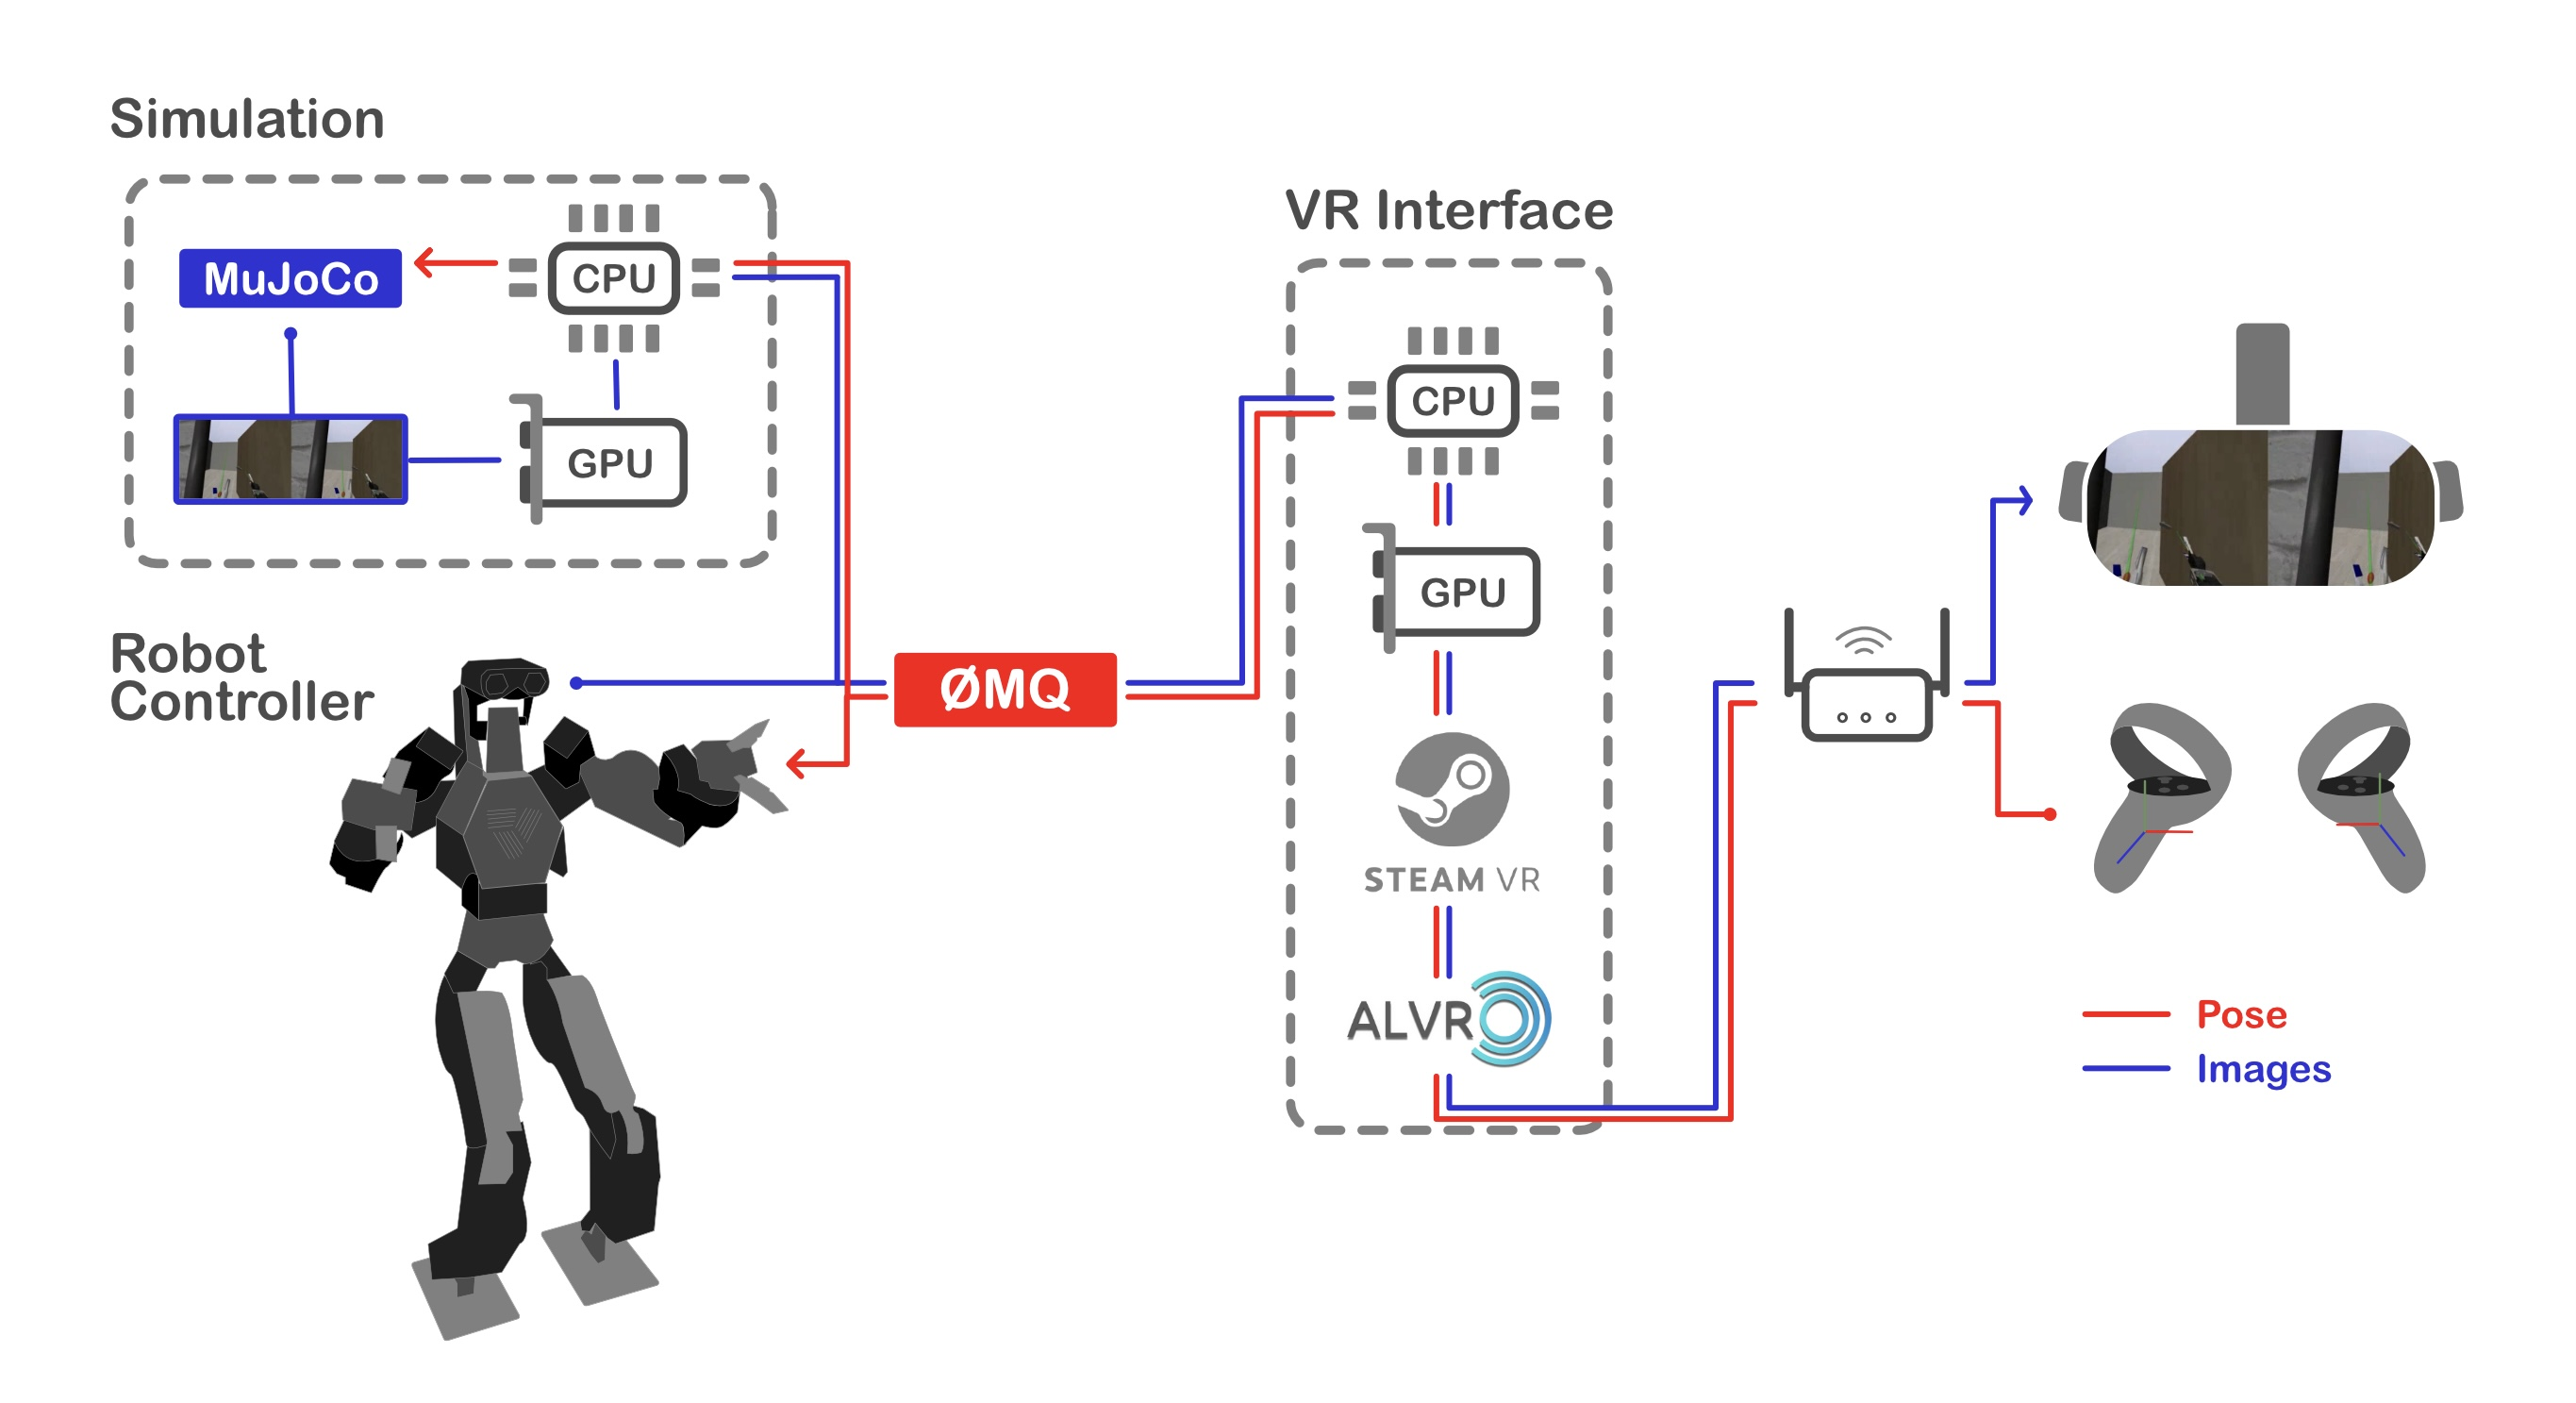
\includegraphics[width=\linewidth]{architecture_diagram.jpeg}
	\caption{Architecture for the VR interface}
    \label{fig:vr-interface}
\end{figure}

Figure \ref{fig:vr-interface} describes the software architecture. The VR interface code written in C++ runs on a separate laptop, which is connected to either the simulation desktop or the robot control station for the real robot. We use OpenVR (implemented in SteamVR) and ALVR (Air Light VR) for the communication between the laptop and the headset. OpenVR is a low-level API for VR applications designed to support a wide range of VR devices. ALVR is an open-source project that allows streaming Steam VR games from the laptop to the headset via Wi-Fi. It implements technologies such as Asynchronous Timewarp and Fixed Foveated Rendering for a smoother experience. ZMQ is an asynchronous messaging library that simplies message-passing between different programs or devices. 

For the simulation, we use Mujoco with Python binding for the physical simulation and Robosuite for the objects in the scene. We first render the scene using a virtual stereoscopic camera that is adjusted to match the interpupillary distance of the VR headset. Then, the rendered pixels are copied from the GPU to CPU and sent to the VR interface using ZMQ and ethernet. The interface code listens to the images and writes them into a GPU texture used by OpenVR. Finally, SteamVR and ALVR transmits the images through a router and displays them in the VR headset. At the same time, the interface polls the VR headset for the poses of the headset and controllers through OpenVR. It transforms the controller poses to the local frame of the headset, and they are then mapped to the poses of the robot hands in the robot's local frame. The latter mapping involves aligning the rotation axes of the controller with the axes used in the simulation. Let $R_t$ be the transformation between the VR axes and the simulation axes, $R_{vr}$ be rotation of the controller from its natural orientation, and $R_{sim}$ be the desired rotation to be applied to the robot hands. Their relation can be expressed as 
$$
R_{sim} = R_t^{-1} R_{vr} R_t
$$
The transformed hand poses are then published continuously using a ZMQ pub socket. When the simulation needs a VR command, it pulls the most recent command from the queue and sends it to the whole-body controller. 

The setup for the real robot is similar. However, since the robot has a lot more components to manage, it will be described in more details in the next chapter.

\section{Design Choices}

Some difficult design decisions were made to satisfy the requirements defined above. They are explained in the section in hopes of providing documentation and guidance for others working on similar systems.

\subsection{OpenVR}

Initially, a website was created based on WebXR and JavaScript to stream controller poses over the internet. I wanted to improve the latency by keeping the connection within a local network, but I encountered difficulty in setting up HTTPS certificates in the campus lab. After getting tired of tunneling the connection over the internet, I decided to pursue a more low-level approach. 
The native Oculus SDK could work, but it would limit the option to change VR systems in the future. Unity is a good option for cross-platform compatibility, but since there's only a need to stream images and controller poses, a game engine is an overkill. I also don't believe that Unity exposes the low-level functionality to directly show the stereoscopic images. Since Unity uses the low-level OpenVR API, I decided to use it directly. Although a newer API called OpenXR is gaining steam, I feel that the performance benefits of OpenXR doesn't justify its complexity compared to OpenVR. 

Using OpenVR has several advantages. First, it has great performance since it is used by VR games and has direct support from VR headset manufacturers. The fact that all SteamVR games use it also makes it suitable for my proposal to embed the demonstration collection system in video games. Second, it delegates the work of video streaming to existing technologies. Many VR headsets support direct HDMI connection from the computer's graphics card, which OpenVR can take full advantage of since it takes input images from OpenGL. Even though the Quest doesn't have an HDMI cable, it is still possible to use the Oculus Link (over an USB cable) or Oculus Air Link (over a local network) with OpenVR. These are sophisticated streaming technologies that predict the user's movements and streaming latency to render ahead of time, and they encode the frames as slices in H.264 \cite{air-link}. ALVR is an open-source alternative that implements similar technologies with the added benefit of having experimental support for Linux. This is much more performant and scalable than hand-coding an image streaming pipeline, as done by \cite{arunachalam2022holodex}. Finally, OpenVR works on a variety of Operating Systems and targets many VR headsets. My code readily runs on Windows laptops just like Linux.

\subsection{Image Transfer from GPU to CPU}

Since our interface script is written in C++ (since the Python OpenVR binding doesn't work well) while the simulation is in Python, we need a way to transfer the rendered images between processes. 
First, we can use memory sharing or pybind to transfer the Mujoco simulation state. Using the simulation states, the C++ code can directly render the scene using Mujoco and pass the result directly to OpenVR within the GPU. However, since Mujoco allocates simulation data structure dynamically, it's difficult to do inter-process memory sharing. Second, we could hypothetically share the GPU buffer rendered by the python script with the C++ script, but OpenGL contexts don't seem to allow inter-process sharing. Third, we can lose some performance and transfer the images from GPU to CPU. Once the images are in memory, we can send them over using ZMQ. 

The last approach was chosen to make the design more adaptable to the real robot, where the images are always coming from memory. The rendered images have a resolution of $1096 \times 2$ by $1176$, where the width is multiplied by 2 to account for both eyes. The rendering of an image takes .3 milliseconds on the RTX3090 GPU, copying it to the CPU consumes 3 milliseconds, and sending it through ZMQ uses .6 milliseconds. Overall, this number is negligible compared to the simulation and whole-body control times, so this performance is acceptable. 

\subsection{Asynchronous Message Passing}

The simulation uses a ZMQ sub socket to get actions from the pub socket in the interface script. Usually this is done synchronously, meaning that the simulation waits for the interface to provide a response after requesting. However, this approach usually takes 70 milliseconds for the message round-trip. This delay can be reduced to .1 milliseconds by using an asynchronous approach. In this case, the sender and receiver simply run at their own pace, and the ZMQ threads in the background takes care of getting the messages ready. When the simulation requests an action, the ZMQ simply gets the most recently received message in its queue and returns it. Since the interface runs at a higher frequency than the simulation, there will never be a case where no action is available. Also, by setting the "conflate" option in ZMQ, we can reduce the need of a queue by only keeping the most recent message. 

\subsection{Separate Computer for VR Interface}

At first, the simulation and interface scripts ran on the same desktop computer. However, we noticed that the scripts were competing for resources, causing performance degradation. We chose ALVR since it's the only option on Linux to connect to VR, and its wireless design enables remote teleoperation. However, encoding the stream in real time consumes CPU power needed for the whole-body controller. When running, the simulation and whole-body controller takes up 1500\% of the CPU, while ALVR and SteamVR consume around 200\%. After decoupling the VR interface to a separate laptop, we noticed around 10\% performance improvement.

\section{Performance Analysis}
The performance of the VR Interface is acceptable. Using asynchronous message passing and a separate laptop for VR interface, receiving images and sending commands are both sub-millisecond operations. The biggest contributor to latency is ALVR, which adds about 70 milliseconds of latency. However, this is nothing compared to the latency introduced by slow simulation. In the simulation loop, for every rendering and communication with the interface, we run 25 simulation steps and 5 whole-body control computations. In comparison, on the hardware, the whole-body control code is run 20 times between every two action inputs. This means that in simulation, the whole-body control code may not have reached the desired action before a new action is given. Indeed, the slow tracking speed of the whole-body control introduces a large delay between the movement of the controller and the robot's hands reaching the desired poses. We qualitatively assessed this by rendering the desired poses as arrows in simulation, and we found that for fast motions, the robot can take up to a second to reach the desired state. 
\begin{figure}
	\centering
	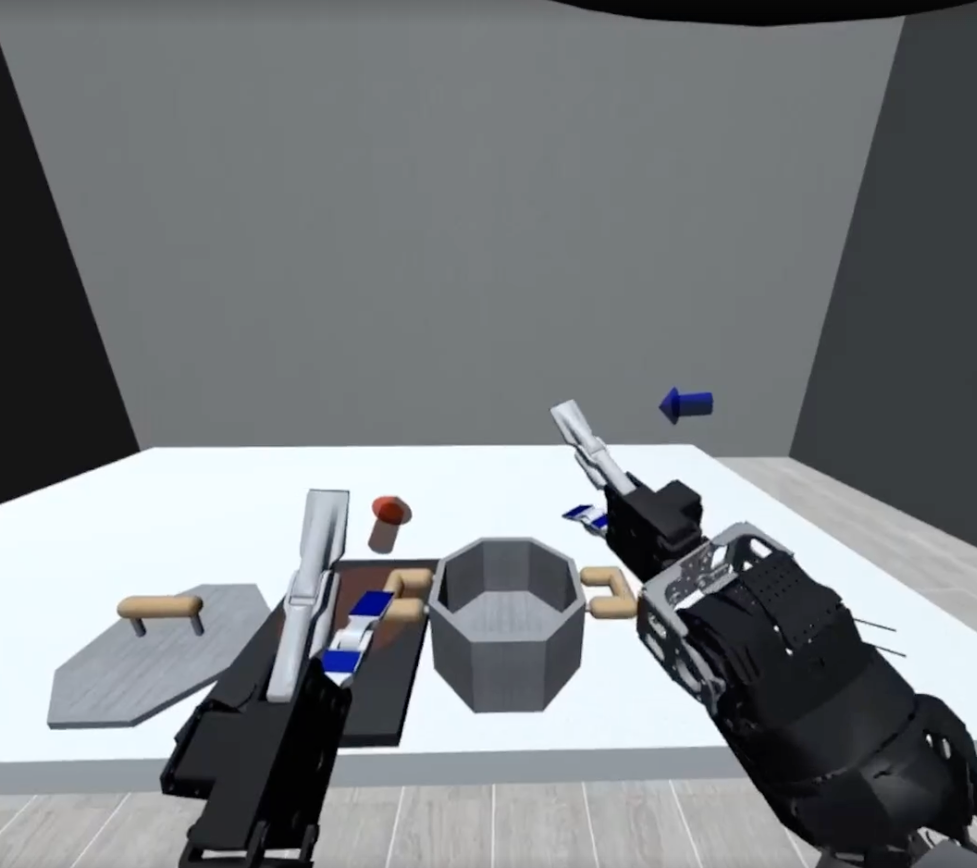
\includegraphics[width=15em]{arrows.png}
	\caption{The robot hands takes time to reach the desired controller poses (represented by arrows).}
    \label{fig:arrows}
\end{figure}

Another big issue with the current setup is speed. The current simulation loop can only achieve around 10 fps in the contact-rich kitchen environment. This is also the reason we can't simply increase whole-body control computation frequency. A humanoid robot capable of walking requires an accurate physical simulation. We are using Mujoco with the RK4 integrator and PGS numerical solver at 50 iterations per time step, where the time step is set at 2 milliseconds. We have also tried running the numerical solver at 10 iterations per time step, sacrificing some precision for speed. For debugging, we also tried rendering the images using OpenCV instead of sending them to the VR headset. Some performance numbers are shown in Table \ref{table:perf}. Since the quickest loop time is 70 milliseconds, there is no hope that our setup can reach 60 fps. From the table, we see that using OpenCV to display images takes quite a lot of time, whereas sending the images to VR is faster. When walking is not involved, the whole-body controller time is reduced drastically, while manipulation tasks involving contact slows down Mujoco. Overall, Mujoco and whole-body control are the biggest culprits for performance issues. 

\begin{table}[h]
\scriptsize
\begin{center}
\caption{Simulation performance numbers. The left column denotes whether OpenCV or the VR headset is used to display the image and the number of PGS iterations per time step. The last row shows a manipulation task without locomotion. In each loop, Mujoco runs 25 times, WBC runs 5 times, and rendering runs once. The first three columns measure the time taken in each run, the fourth column shows the total time taken by each loop, while the last three columns show their percent contribution to total loop time considering the number of times they run.  }
\vskip 10pt
\begin{tabular}{|c|c|c|c|c|c|c|c|}
\hline
& Mujoco (ms) & Render (ms) & WBC (ms) & Total (ms) & Mujoco & Render & WBC\\
\hline
	CV, 50 & 1.72 & 30 & 7.7 & 120 & 35\% & 27\% & 31\% \\
\hline
	CV, 10 & .8 & 30 & 7.7 & 100 & 21\% & 33\% & 39 \% \\
\hline
	VR, 50 & 1.72 & 8 & 6 & 92 & 48\% & 8\% & 34\% \\
\hline 
	VR, 10 & .92 & 8 & 6 & 70 & 33\% & 11\% & 44\% \\
\hline 
	
	\begin{tabular}[x]{@{}c@{}}VR, 50\\no walking\end{tabular}& 2.12 & 8 & 5 & 90 & 57\% & 8\% & 25\%\\
	\hline
\end{tabular} \\[10pt]
\vskip -20pt
\end{center}
\label{table:perf}
\end{table}


However, this is not the end of the story for potentially embedding our setup in a video game. As mentioned, our simulation codebase is written in Python. When the C++ codebase from the hardware team is used, each WBC computation is reduced from 5 to .45 milliseconds. In fact, the hardware team has their own simple simulation in PyBullet for debugging purposes. As mentioned before, they run 20 simulation steps and 20 WBC calls per loop. On the same machine, their loop is able to execute 40 times per second with the VR interface. Needless to say, one of our current tasks is to substitute our Python code with their C++ code.

\chapter{Real-Robot Experiments}

In this chapter, the details of how our experiments are conducted on the real robot are introduced. 
However, due to the complexity of the robot system, the infrastructure built for collecting demonstrations and deploying the neural network policy will be described first. Specifically, a real-time system was build to integrate the camera, grippers, whole-body controller, and the VR headset. Then, the data collection and neural network policy evaluation results (or lack of thereof) are discussed. 

\section{Infrastructure}

\begin{figure}
	\centering
	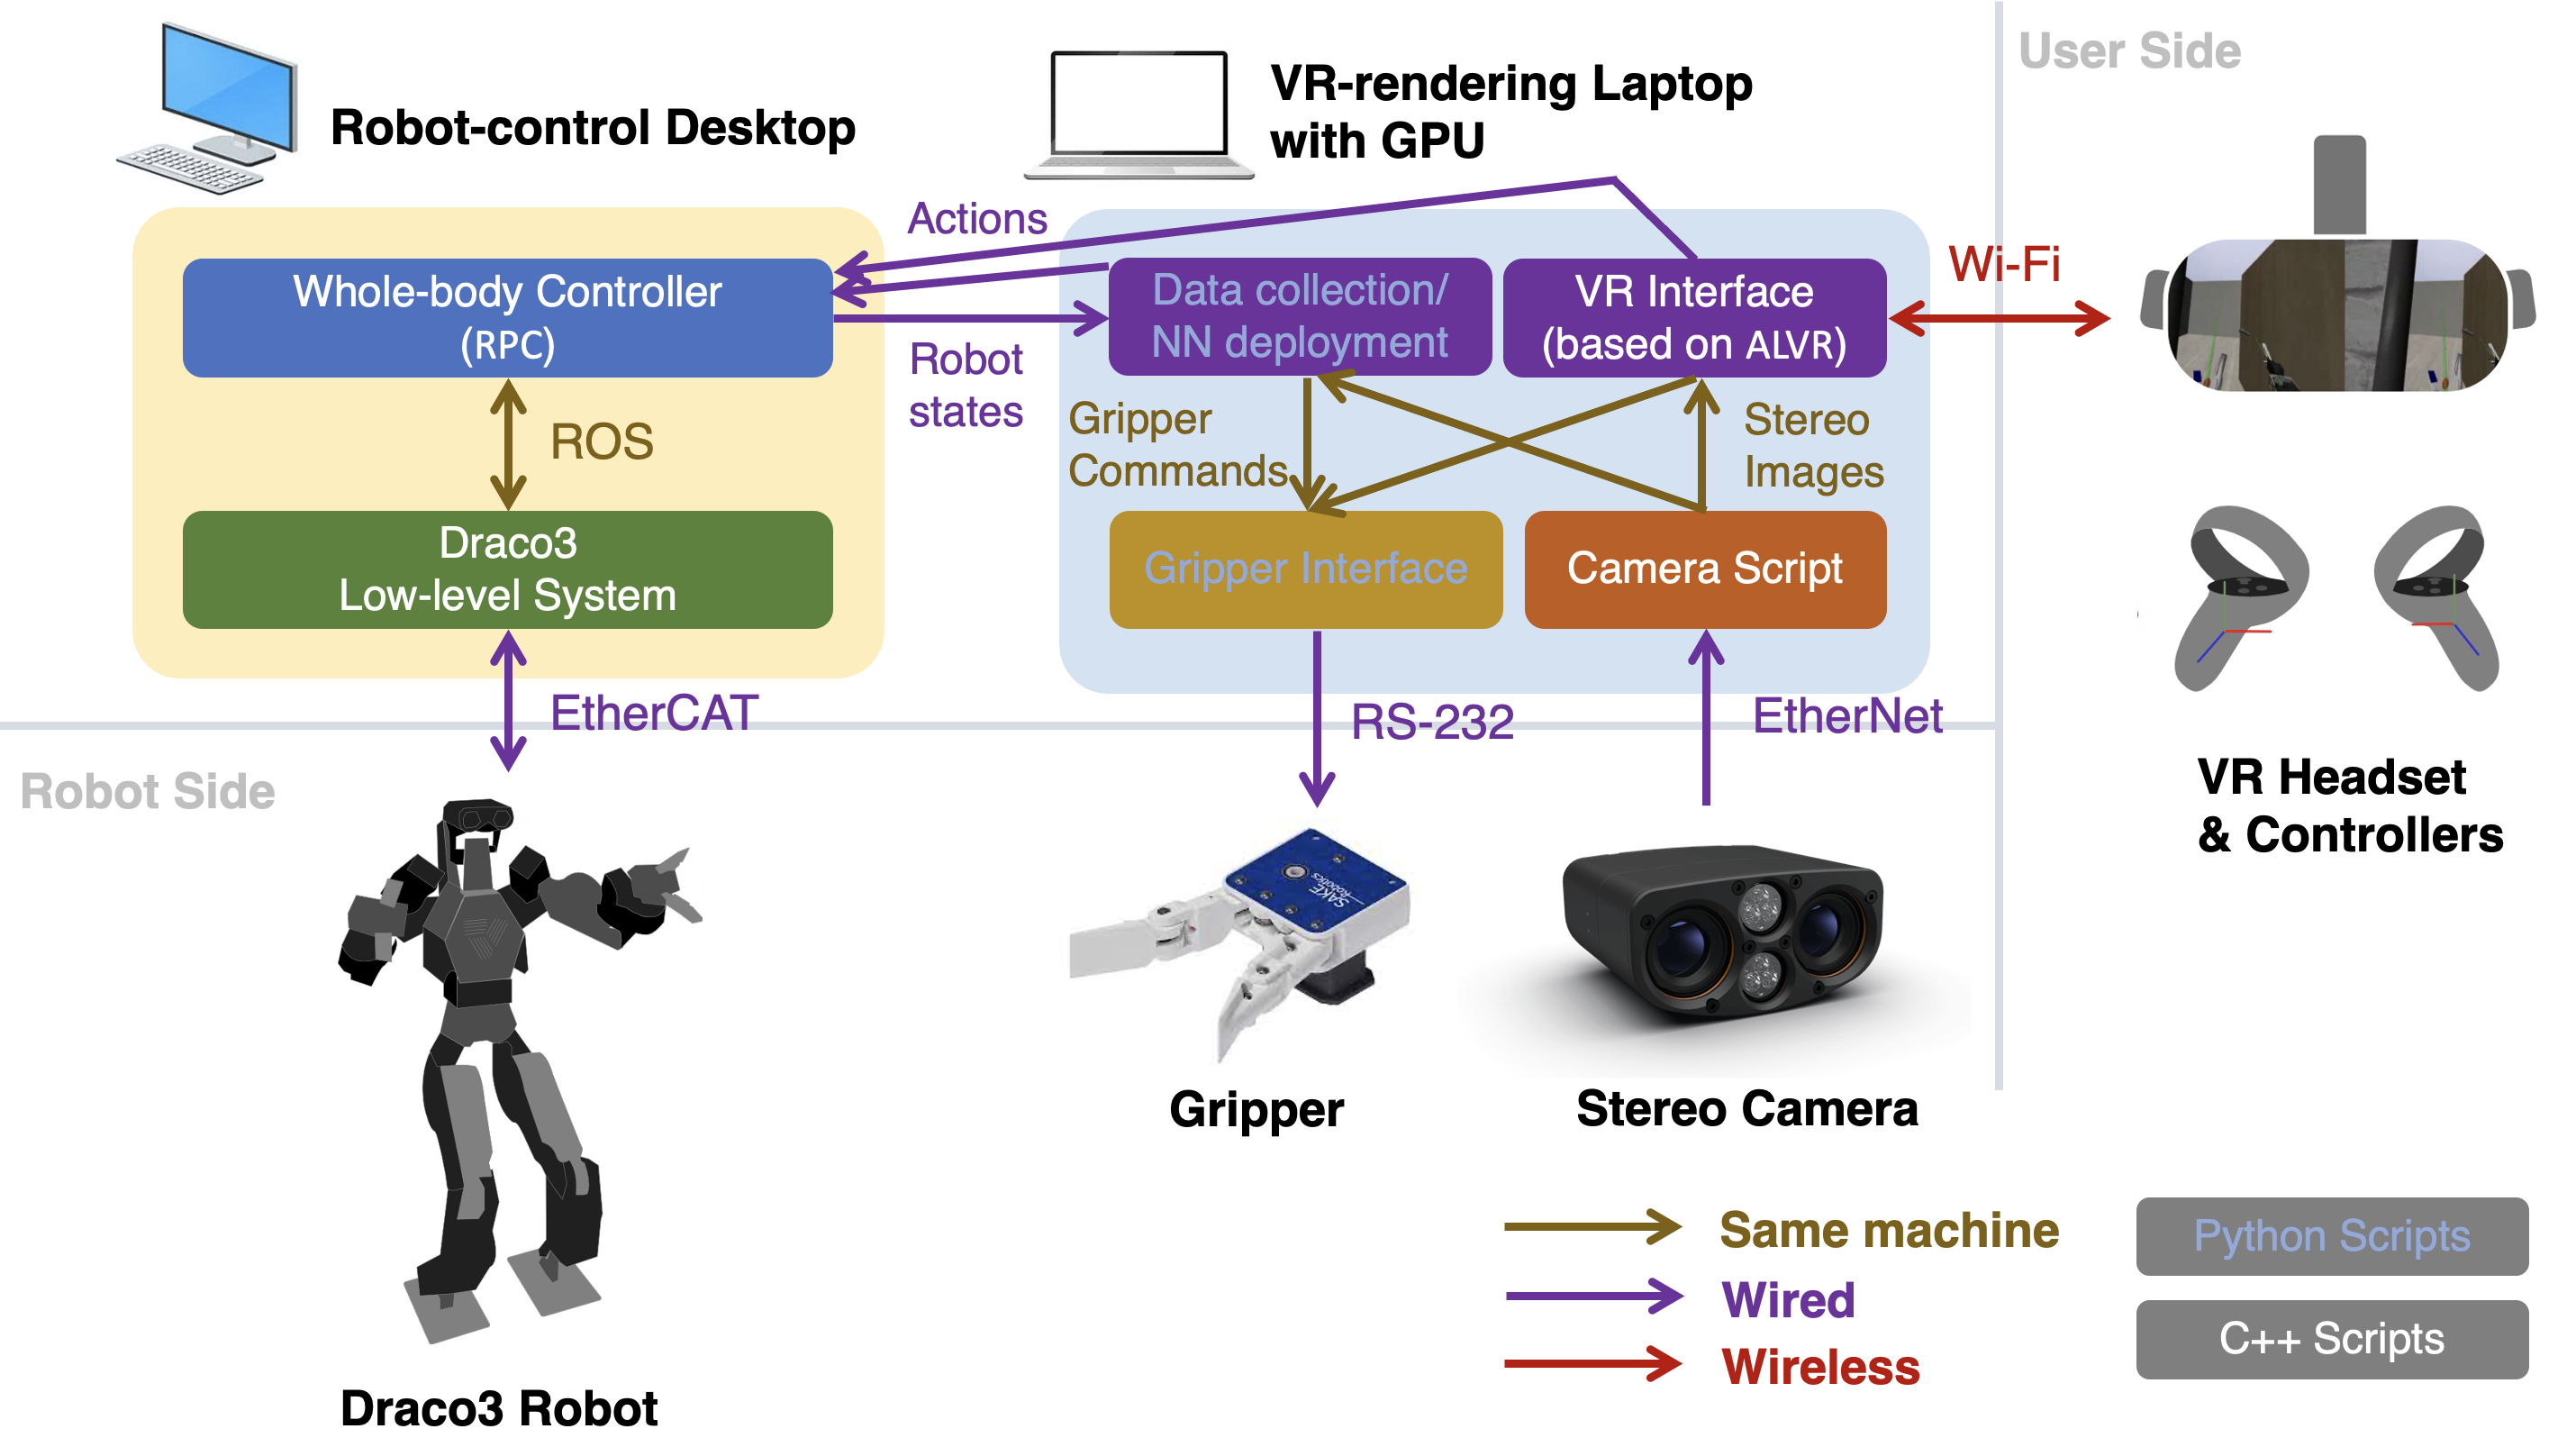
\includegraphics[width=\linewidth]{robot-architecture.png}
    \caption{The infrastructure used to collect demonstraions and deploy policy on the real robot. Original diagram by Mingyo.}
    \label{fig:robot-architecture}
\end{figure}

Figure \ref{fig:robot-architecture} shows the infrastructure for collecting demonstrations and deploying trained policies on the real robot. 
The VR Interface script is the same as before, but more components are added to interface with the grippers, camera, and the robot-control desktop. The whole-body controller running on the desktop is a modified version of PnC \cite{Ahn2021VersatileLP}, named RPC (Robot Planning and Control), created by the hardware team. 

When collecting demonstrations, the camera footage is streamed from the robot's stereo camera to the VR headset. Both RPC and the gripper interface subscribe to VR commands to execute desired actions. The data collection script then pulls robot states from RPC and camera footage from the camera script and saves the resulting data into an HDF5 file. The saved data is then post-processed and used to train the neural network. 
During deployment, the observations (robot states and camera footage) are processed in real-time and fed into the neural network. The processing involves converting hands and feet poses to local frame of the robot and normalizing and resizing images. Then, the neural network inference is performed on the GPU laptop, and the output commands are issued to the grippers and robot. The output commands are restricted by a 3D bounding box to prevent extreme values that can damage the robot. 

\subsection{Streaming Images From Camera to VR}

Unlike simulation, the parameters of the camera on the robot cannot be easily adjusted. This means that the interpupillary distance and FOV of the camera does not match those of the human eyes, causing dizziness in the demonstrator \cite{distortion}. Although cropping the images helps with adjusting the convergence distance of the cameras, the difference in interpupillary distance cannot be completely fixed. In addition, there is only RGB data from the left camera, whereas the right camera only has grayscale images. Instead of colorizing the right image from the left image using computer vision techniques, which can produce artifacts that are easily noticeable by the human, we opted to only display grayscale images in the headset. Although the experience isn't very smooth, the depth perception provided by stereoscopic images is still enough to complete many manipulation tasks with relative ease. 

The camera is the MultiSense S7 model from Carnegie Robotics. It comes with a low-level driver library with minimal documentation. RGB image streaming is achieved by executing callback handlers for luma and chroma images on separate threads and merging them together into RGB. Similarly, left and right luma images are streamed in separate threads, which are then synchronized and stitched together to form stereoscopic images. This multi-threaded C++ code is designed to incur minimal image-copying and is thus very efficient.

\section{Neural Network Training and Evaluation}

Our Neural Network takes in the following inputs: stereoscopic images resized to 800x200, positions and velocities of the 26 joints in sin and cos form, the SE(3) poses of the hands and feet in local frame, and the current state machine of the robot, such as balancing or walking forward. A Resnet is trained to extract the image features, and a RNN is used to process the features as well as other inputs to produce an output distribution. The continuous outputs such as hand trajectories are fed into a GMM to produce manipulation commands, while discrete outputs such as locomotion commands and grippers are rounded to either 0 or 1. 

\begin{figure}
	\centering
	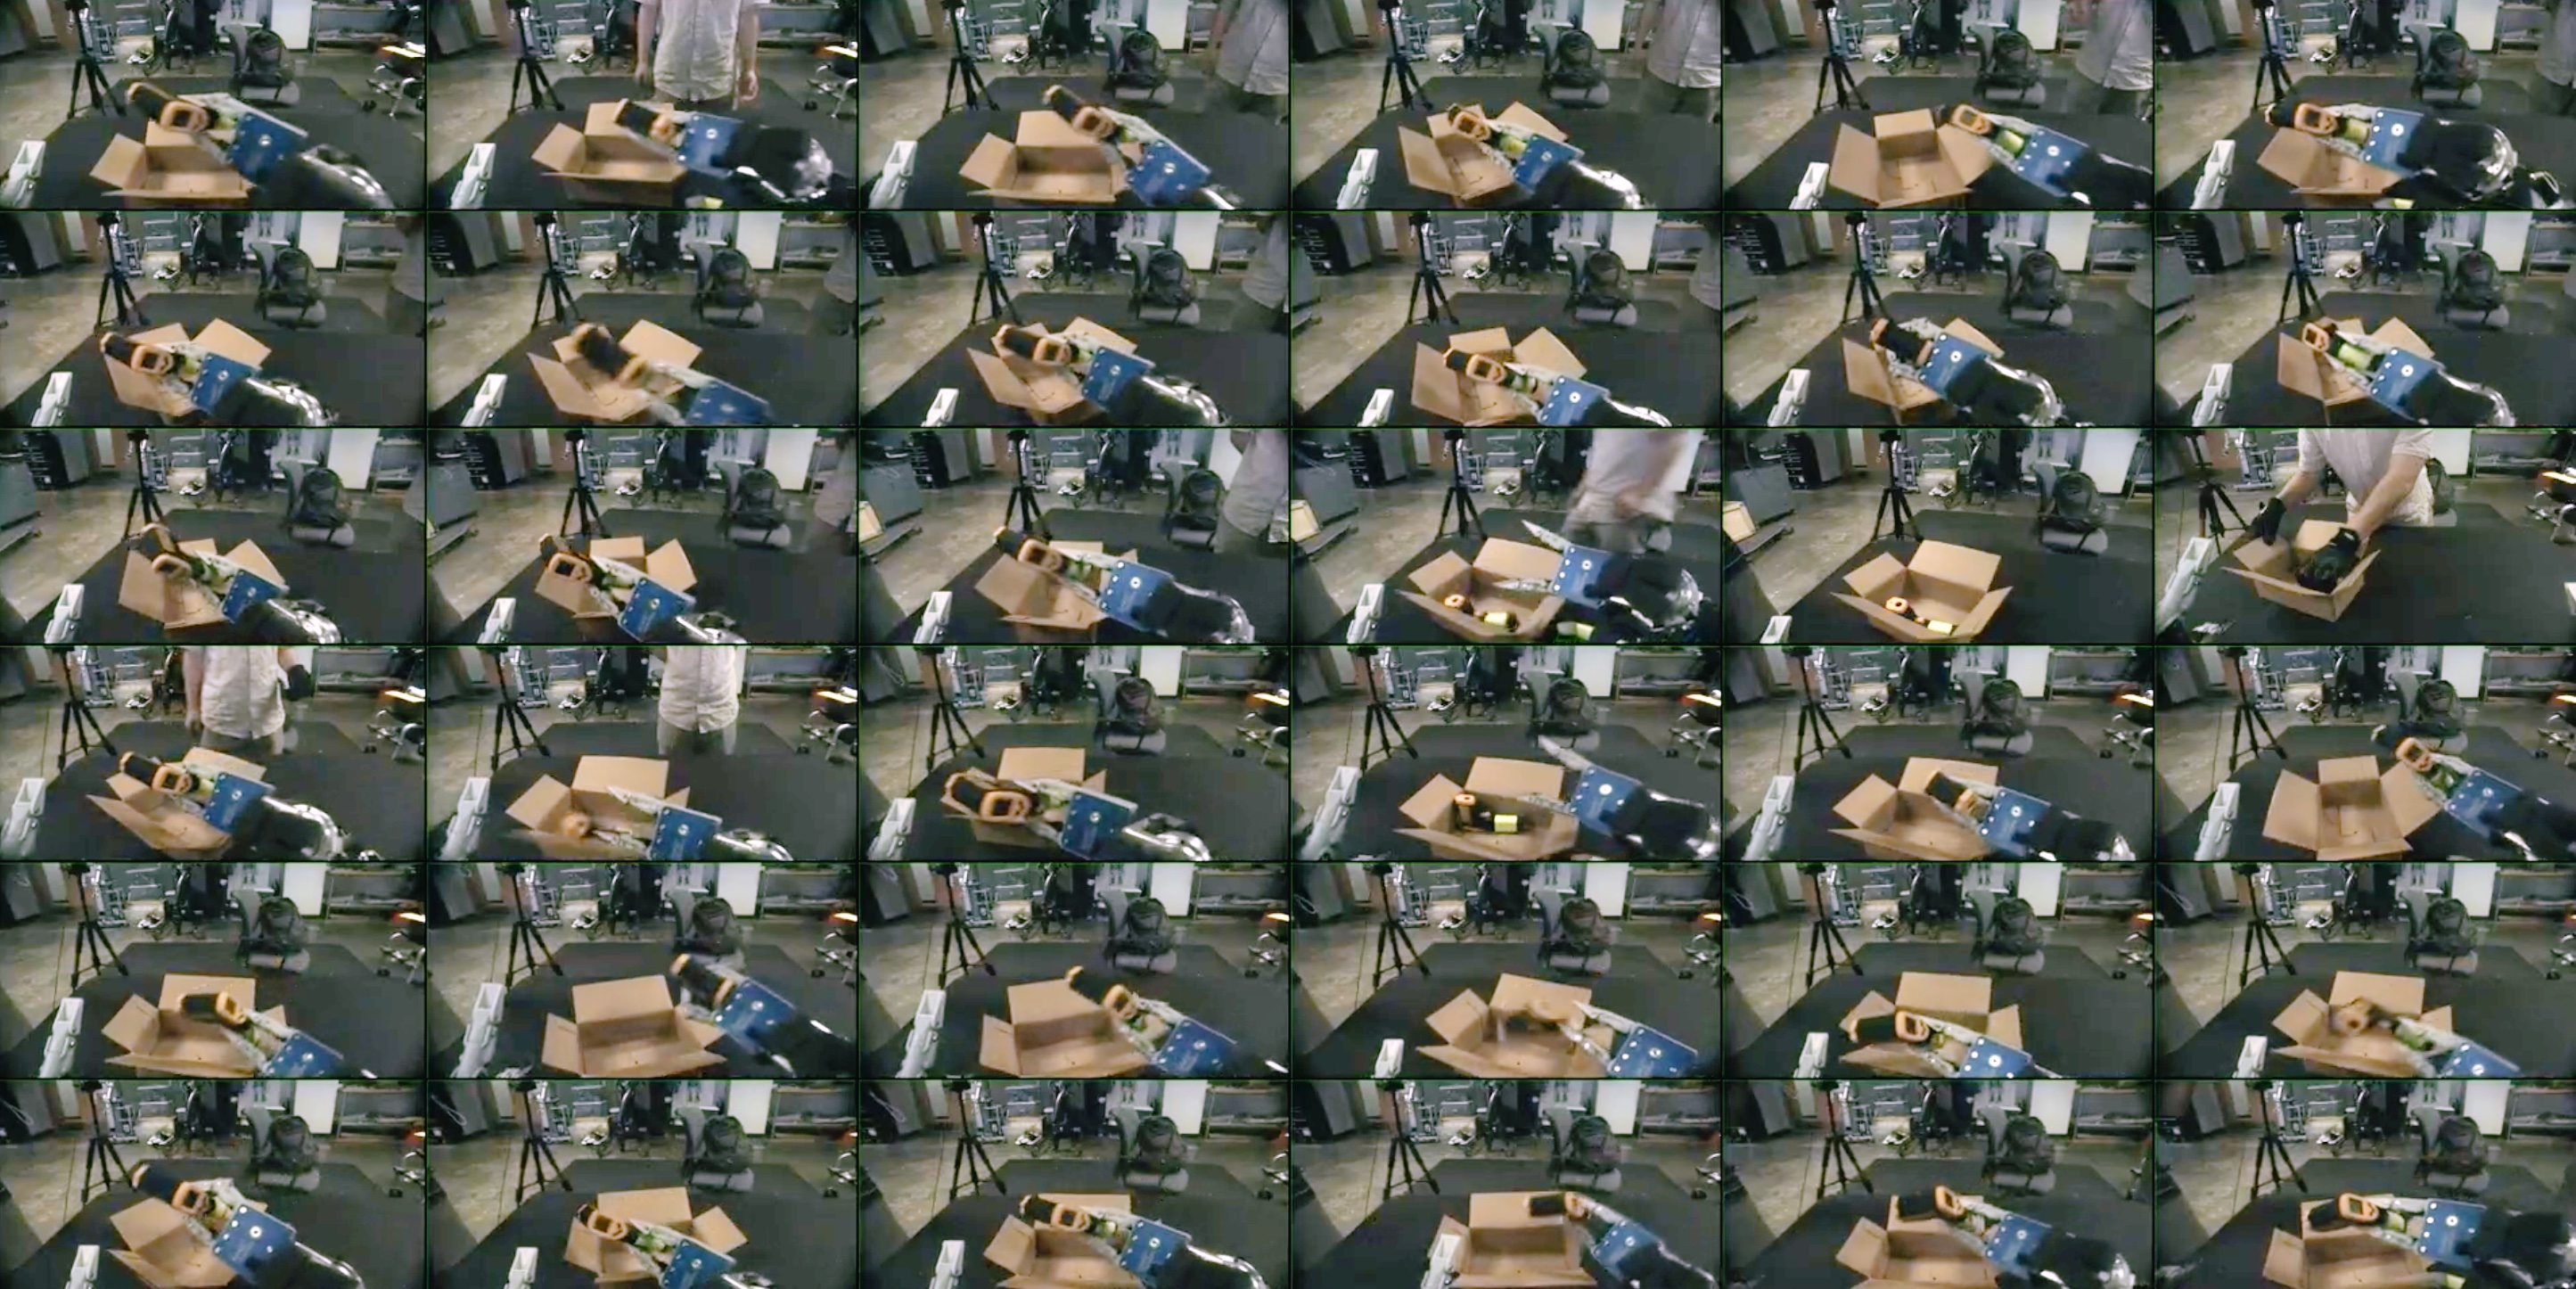
\includegraphics[width=\linewidth]{pick-and-place.jpeg}
    \caption{150 demonstrations of a simple pick-and-place task are collected. The egocentric view for some of the episodes are shown. }
    \label{fig:pick-and-place}
\end{figure}

To train the network, 150 demonstrations are collected on a simple pick-and-place task involving grabbing a temperature gun and dropping it in a box, as shown in Figure \ref{fig:pick-and-place}.

\begin{figure}
	\centering
	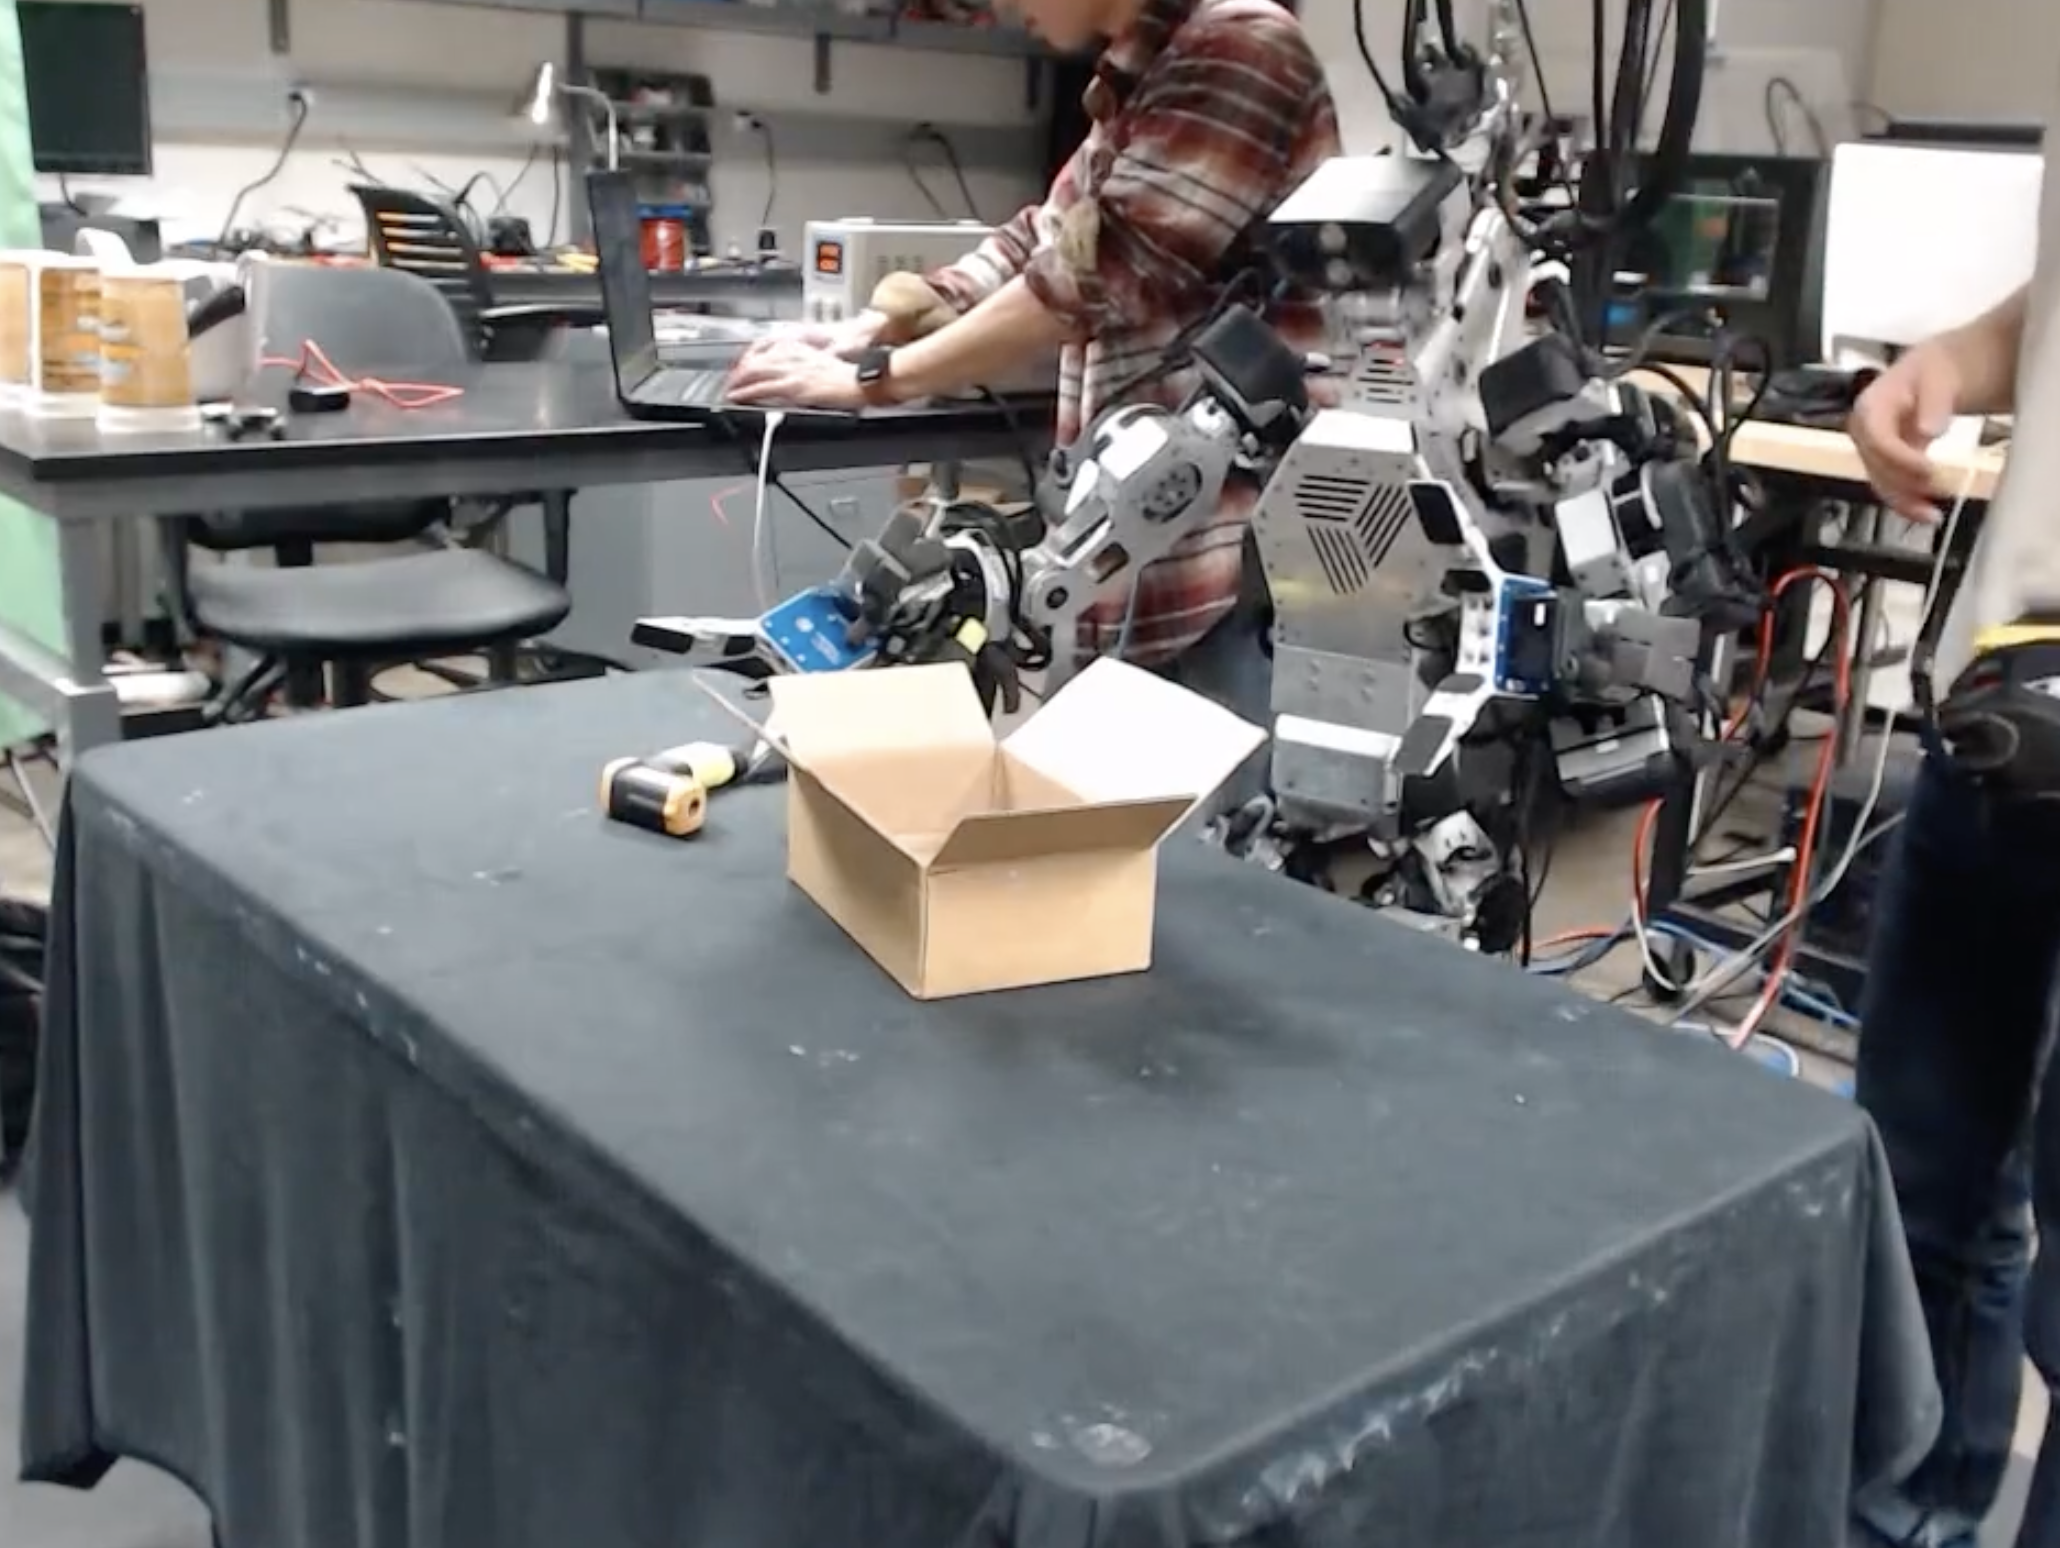
\includegraphics[width=20em]{real-eval.png}
    \caption{During evaluation, the robot usually knocks over the temperature gun before grasping it.}
    \label{fig:real-eval}
\end{figure}
\begin{figure}
	\centering
	\includegraphics[width=\linewidth]{"Right hand orientation.png"}
	\includegraphics[width=\linewidth]{"Right hand position.png"}
    \caption{Plotting the desired vs actual position and orientation of the right hand during deployment. }
    \label{fig:tracking-plot}
\end{figure}


However, the evaluation of the trained policy is not very successful. Out of 20 evaluations, the robot is only able to pick up the temperature gun in 1 episode. As shown in Figure \ref{fig:real-eval}, the robot fails to locate the object and often knocks it over. 
We hypothesize that the tracking error of the whole-body controller is partially reponsible for the difficulty to learn precise manipulation. Figure \ref{fig:tracking-plot} shows tracking error of the right hand during deployment.


We are currently working on debugging this issue, but unfortunately, due to the frequent need to repair the robot (see Figure \ref{fig:surgery} for one of the many robot "surgeries"), we are not able to solve it by the thesis due date. The difficulty of performing real-robot experiments on a humanoid platform is the very reason we started out with simulation. Indeed, we have gotten much better results in simulation.

\begin{figure}
	\centering
	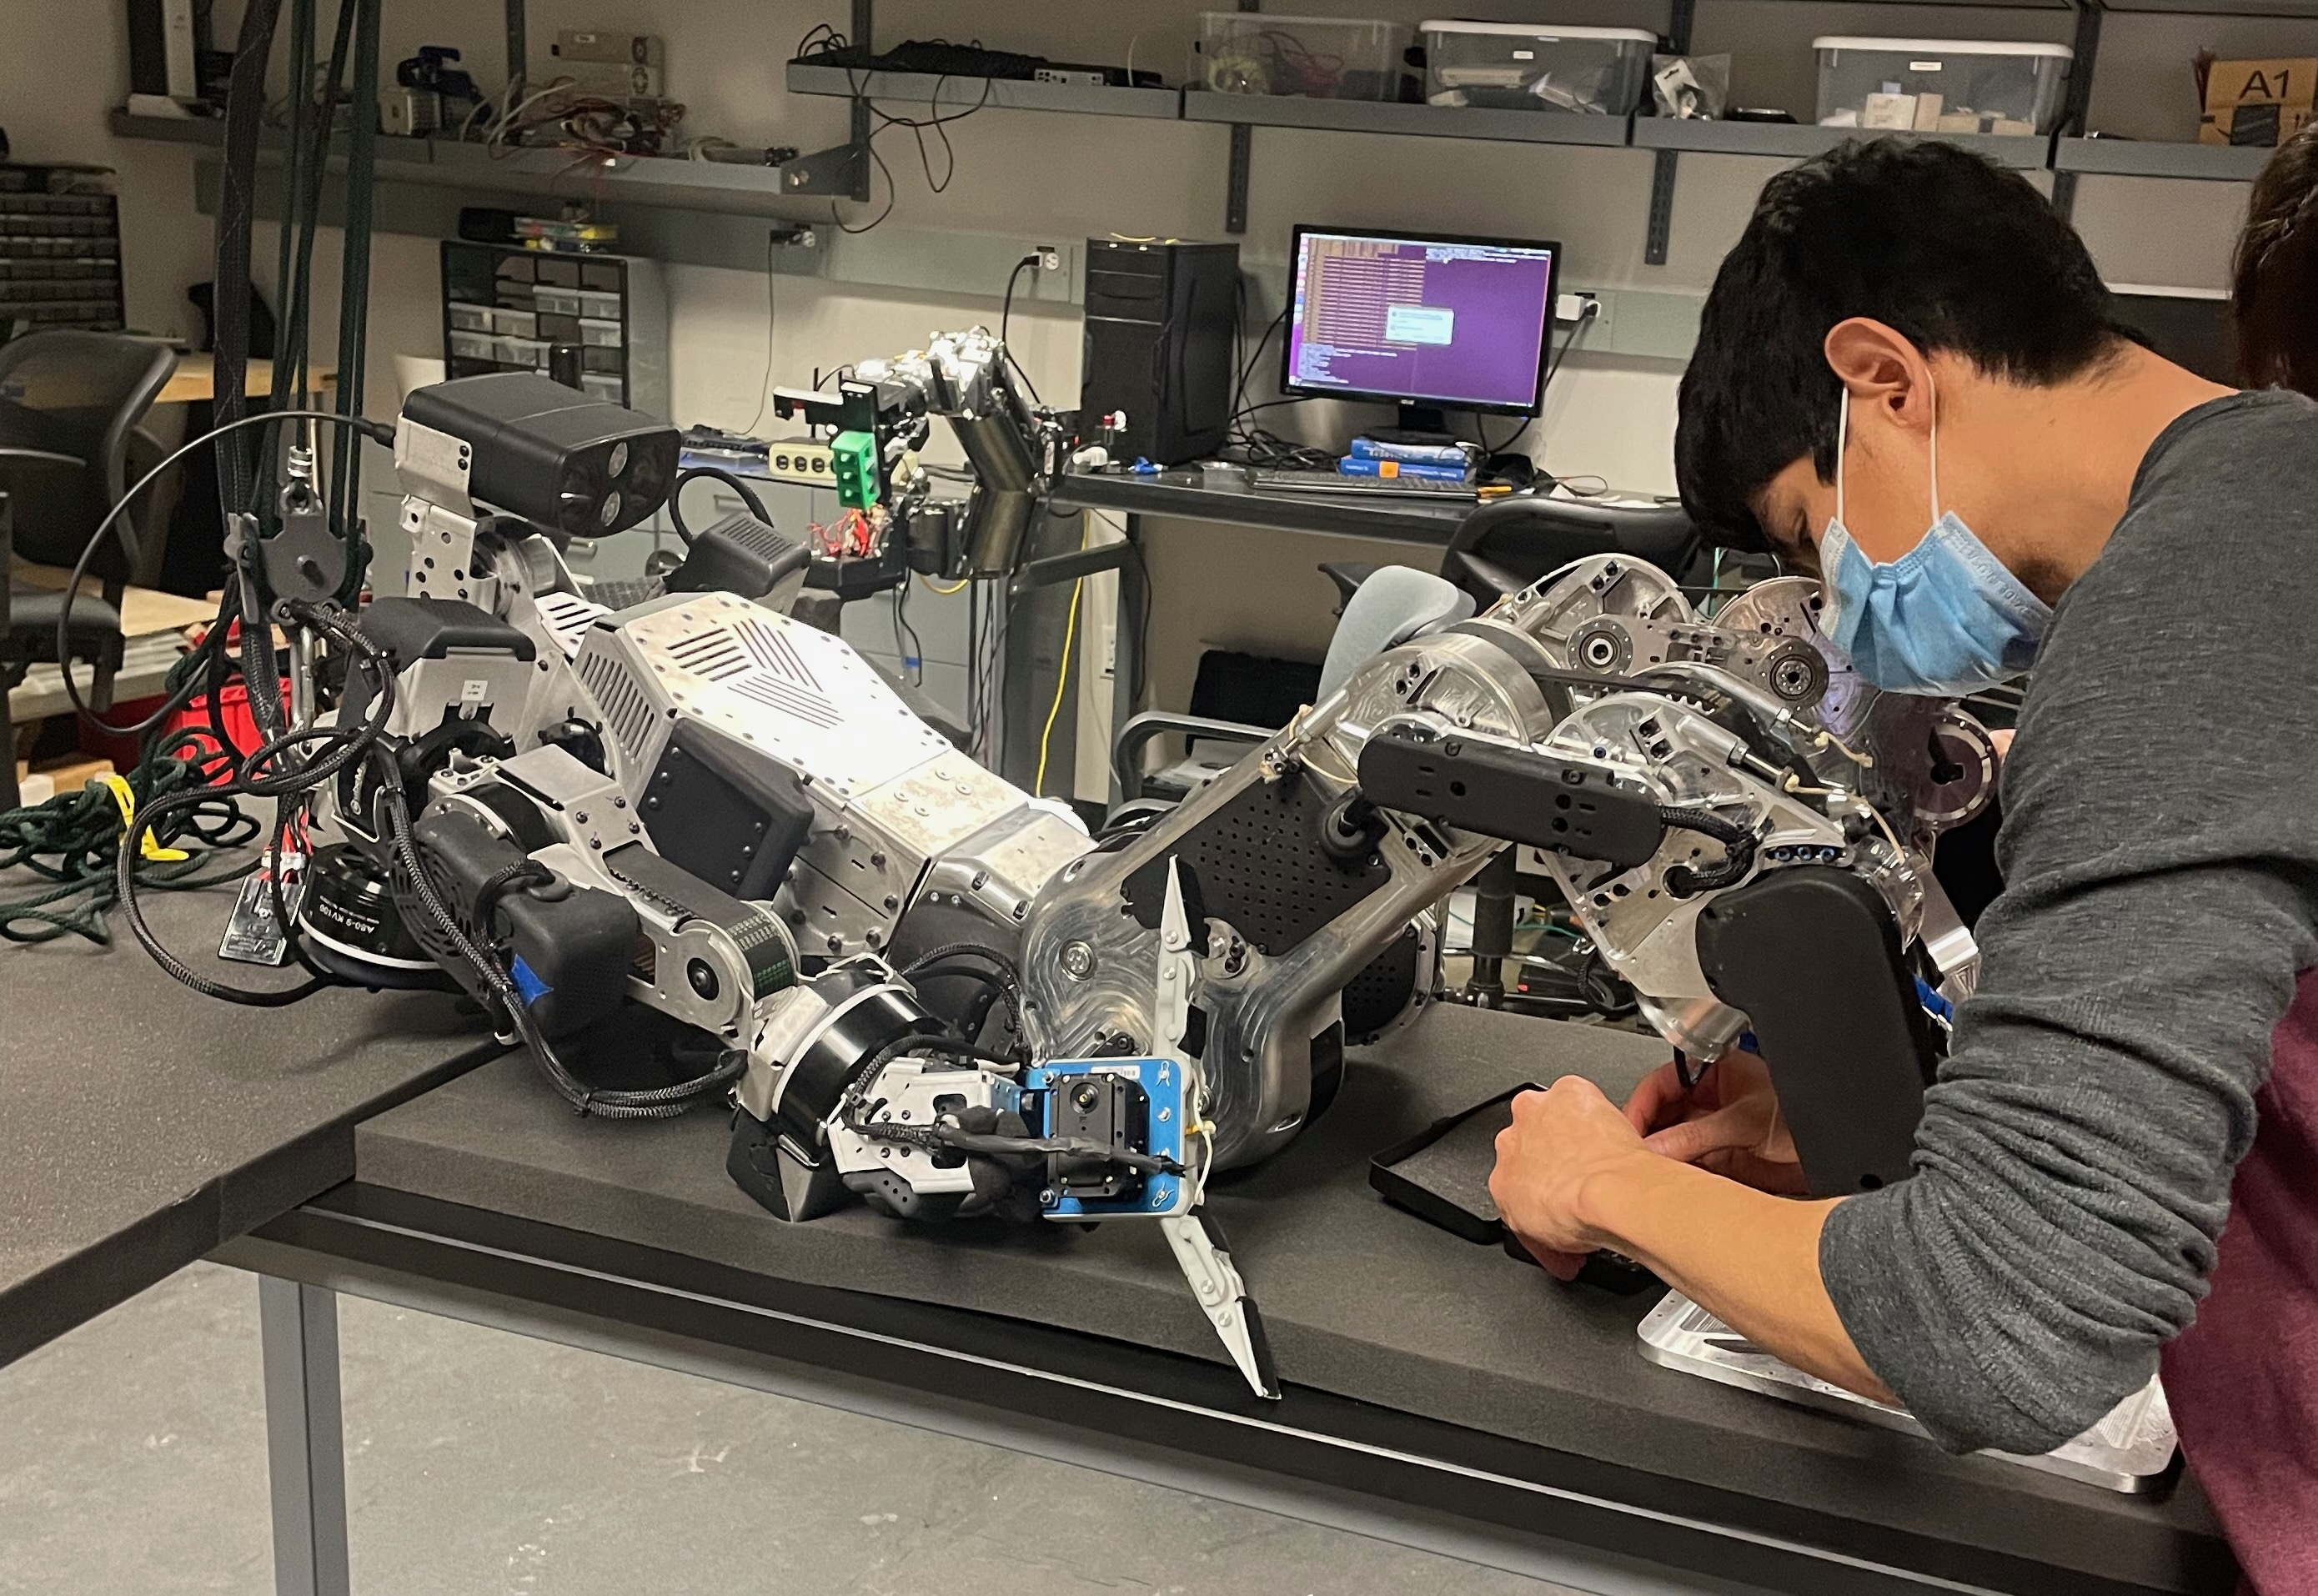
\includegraphics[width=20em]{surgery.jpeg}
    \caption{During one the experiments, a rod end on the robot's ankle broke. Mingyo created a simulation to test out algorithms since hardware experiments are expensive. }
    \label{fig:surgery}
\end{figure}

\chapter{Simulation Experiments}

In this section, the tasks used in simulation experiments and the results are presented. 

\section{Tasks}

The first environment is a door in a hallway. For the first task, the robot needs to grab the handle, turn it, and push the door open. The second task is a loco-manipulation task, where the robot needs to walk forward and push the door open. 

The second environment is a kitchen. 

\chapter{Future Work}

Immersive demonstration with force feedback 

https://arxiv.org/pdf/2301.09157.pdf

training techniques used in VR fixed-base

representation learning holodex


%\chapter{Instructions for Preparing Dissertations, Theses, and Reports}
\index{Instructions for Preparing Dissertations, Theses, and Reports%
@\emph{Instructions for Preparing Dissertations, Theses, and Reports}}%

We are not going to look at the complete set of instructions contained
in \emph{Instructions for Preparation of Doctoral Dissertations and
Dissertation Abstracts} or \emph{Format For The Master's Thesis and Report}
which can be obtained from the Office of Graduate Studies (OGS)
\index{Office of Graduate Studies}%
or on their web page,
\index{Office of Graduate Studies web page}%
\url{http://www.utexas.edu/ogs}.
The doctoral Instructions I am using are dated March, 2001.
The master's Format I am using is dated May, 2001.

Here we will look at a few instructions related to the arrangement of the
dissertation, thesis, or report and a few other ``technical'' details,
providing some examples of common \LaTeX\ usage and some examples of
not-so-common \LaTeX\ usage.

The following are just a couple of tests for the ``quote''
and ``quotation'' environments. The following paragraph is a quote.
\begin{quote}
\index{quote}%
This template package is provided and licensed
``as is'' without warranty of any kind, either expressed or
implied, including, but not limited to, the implied warranties
of merchantability and fitness for a particular purpose.
\end{quote}
The following paragraph is a quotation.
\begin{quotation}
\index{quotation}%
This template package is provided and licensed
``as is'' without warranty of any kind, either expressed or
implied, including, but not limited to, the implied warranties
of merchantability and fitness for a particular purpose.
\end{quotation}

The OGS Instructions say prose quotations over four lines
should be indented on the left. The Doctoral Degree Evaluator says
the quote environment is the correct one to use.

\section{Arrangement of Dissertation}
\index{Arrangement of Dissertation@\emph{Arrangement of Dissertation}}%

Always remember that this ``fake'' dissertation 
\index{fake dissertation}%
is only intended to be a template for writing your own. Since the ultimate
responsibility of making sure your dissertation meets the Graduate School's
requirements, however, lies only with you, you \textbf{\textit{must}} get
the current \emph{Instructions for Preparation of Doctoral Dissertations and
Dissertation Abstracts} from the Office of Graduate Studies or their web
page and check everything yourself. If you don't, you may have a very
rude awakening from the Lynn Renegar, Doctoral Degree Evaluator (aka,
``The Ruler Lady'') at a most inopportune time.

Arrange your dissertation as follows (all sections are required 
unless said otherwise.

\begin{enumerate}

\item Fly Page 
\index{Fly Page}%
(blank protective page). This page is \textbf{not} counted in the numbering.
\textbf{Note:} This template does not insert a Fly Page; if you are printing
an official copy, you must manually insert a blank piece of paper on your own.
Electronic documents do not need a fly page.

\item Copyright Legend 
\index{Copyright Legend}%
(optional) - See OGS Instructions Sample Form A.
Begin counting \textbf{pretext} pages here, but \textbf{do not
place a number on this page.} 

\item Committee Certification of Approved Version.
\index{Committee Certification of Approved Version}%
See OGS Instructions Sample Form B. This page is included in the
pretext count, but there should be no page number on the page.

\item Title Page - 
\index{Title Page}%
See OGS Instructions Sample Form C.
This page is counted, but there should not be a page number on this page.

\item Dedication 
\index{Dedication}%
and/or Epigraph (optional). 
\index{Epigraph}%
Included in count, but not numbered.

\item Acknowledgments
\index{Acknowledgments}%
or Preface 
\index{Preface}%
(optional) - Begin showing \textbf{pretext} page numbers with \textbf{lower
case Roman numerals} at bottom of page.

\item Abstract 
\index{Abstract}%
(optional) - See OGS Instructions Sample Form D.

\item Table of contents -
\index{Table of contents}%
List ALL sections which follow it. There are too may different ways a table
of contents may be done for the OGS to give examples in their Instructions
booklet, but do be sure there is agreement between the major headings in
your text and their designations in the Table of Contents (fortunately \LaTeX{}
does this for you automatically). Please ask the Doctoral Degree Evaluator
for assistance if necessary.

\item List of Tables,
\index{List of Tables}%
List of Figures,
\index{List of figures}%
List of Illustrations, 
\index{List of Illustrations}% 
Nomenclature,
\index{Nomenclature}%
List of Supplemental Files (such as multimedia files)
(optional).

\item Text. 
\index{Text}%
The text should be divided into chapters, books or sections. The first page
is Arabic numeral \textbf{``1''}. All sections, \textbf{from the first page
of text through Vita,} should be numbered consecutively.

\item If you group all Tables, 
\index{Tables}%
Figures, 
\index{Figures}%
or Illustrations 
\index{Illustrations}%
in one place in your dissertation, the section should be placed 
here, immediately after the text and before any appendices 
(optional).

\item Appendix or Appendices 
\index{Appendix}%
\index{Appendices}%
(optional).

\item Glossary 
\index{Glossary}%
(optional) - this section may be placed either here or after the Table
of Contents, in the area with List of Tables, List of Figures...

\item Bibliography
\index{Bibliography}%
- consult your supervisor about which recognized style to use.

\item Index
\index{Index}%
(optional).

\item Vita -
\index{Vita}%
This should be a brief biographical sketch of the author. List in the
Table of Contents. See OGS Instructions Sample Form E.


\end{enumerate}


\section{Other Requirements}
\index{Other Requirements@\emph{Other Requirements}}%


\subsection{Margins}
\index{Margins@\emph{Margins}}%

The dissertation, after printing, should have left and top margins of
1~1/2 inches, and the right and bottom margins should be 1~1/4 inches.
These margins should be consistent throughout the dissertation - including
all pages in the appendix. \textbf{All page numbers must be \textit{at
least} one inch from the edges of the page}. Headers are rarely used in
dissertations; if you are considering using them, check with the Doctoral
Degree Evaluator first to be sure they will be accepted.


\subsection{Spacing and Page Arrangement}
\index{Spacing and Page Arrangement@\emph{Spacing and Page Arrangement}}
\index{Spacing}%
\index{Page Arrangement}%

The document should be double-spaced or space-and-a-half. 
Exceptions to double-spacing are: the Table of Contents, Lists of Tables, 
Tables, Figures, Graphs, Captions, Footnotes, Endnotes, 
Appendices, Glossary, Bibliography and Index; these may 
be single-spaced. Paragraph indentations are usually five to ten 
spaces. Prose quotations over four lines should be in 
block quote (double or single spaced, indented on the left). 
Do not use quotation marks if the quotation is indented except for
quotations within the block quote. Please refer to a style manual for
more detailed instructions.

Be sure that each new chapter or major section (i.e., Appendix, Bibliography,
Vita) begins on a new page.

\section{Master's Theses and Reports}

Always remember that this ``fake'' thesis or report 
\index{fake thesis or report}%
--- assuming you have followed the instructions in the next chapter about
how to format it as such --- is only intended to be a template for writing
your own. Since the ultimate responsibility of making sure your thesis or
report meets the Graduate School's requirements, however, lies only with
you, you \textbf{\textit{must}} get the current \emph{Format For The
Master's Thesis and Report} from the Office of Graduate Studies or their web
page and check everything yourself. If you don't, you may have a very
rude awakening from the Mike Feissli, Master's Degree Evaluator at a most
inopportune time.

That said, the formatting requirements for Dissertations and Reports and
Theses are very similar. They are, however, \textbf{\textit{not}} identical.
The primary differences are in the ordering of the title and signature
pages and where the optional index is inserted. For Master's Theses
and Reports, the Title Page must be in front of the Signature Page. For
Master's Theses and Reports, \textbf{\textit{nothing}} is permitted to
come between the bibliography and the vita; the index, if used, must be
before the bibliography. If you want to use an index, talk with Mike
Feissli before your deadline to verify that its inclusion is
acceptable. The index can be removed by commenting out one line with a
percent sign, if necessary, for producing the ``official'' copy of your
thesis or report, and then inserted for copies for your advisor and
you by removing the percent sign.



%\chapter{Making the Bibliography with BiB\TeX{}}\label{c:bib}
\index{Making the Bibliography with BiBTeX%
@\emph{Making the Bibliography with BiB\TeX{}}}%

BiB\TeX{} 
\index{BiBTeX@BiB\TeX{}}%
allows one to generate automatically the bibliography 
from a database of bibliographic 
items. You need to do the following:

\begin{enumerate}
\item Create the bibliographic database, 
\index{bibliographic database}%
which is a file whose name ends in \texttt{.bib}. 
\index{.bib@\texttt{.bib}}%
Let us call it \texttt{diss.bib}. Entries in this file are like this:
\begin{verbatim}
@BOOK{knuth:tb,
  author = "Donald K. Knuth",
  title = "The \TeXbook",
  publisher = "Addison-Wesley",
  year = "1984",
}
@TECHREPORT{poorten:sp,
  author = "Alf~J.~van der Poorten",
  title = "Some problems of recurrent interest",
  institution = "School of Mathematics and Physics,
                 Macquarie University",
  address = "North Ryde, Australia 2113",
  number = "81-0037",
  month = "August",
  year = "1981",
}
@ARTICLE{erdos:oap,
 author = "Paul Erd{\"o}s and Paul Turan",
 title = "On a problem in the theory of uniform 
          distribution, {I}", 
 journal = "Indag. Math.",
 volume = "10",
 year = "1948",
 pages = "370--378",
}
\end{verbatim}

\item Include a \cn{bibliographystyle} 
\index{commands!bibliographystyle@\cn{bibliographystyle}}%
command in your \LaTeX{} file, say 

\cn{bibliographystyle\{plain\}} 
and a \cn{bibliography} 
\index{commands!bibliography@\cn{bibliography}}%
command to load the bibliography, 
in this case \cn{bibliography\{diss\}}, at the point of your 
document where the bibliography should be inserted. 

The document at this point will look like this:
\begin{verbatim}
\bibliographystyle{plain}
\bibliography{diss}
\end{verbatim}

\item Run \LaTeX{} on your main file, say \texttt{foo.tex}: 
\texttt{latex foo}. This generates an auxiliary file 
\texttt{foo.aux} with a list of \cn{cite} 
\index{commands!cite@\cn{cite}}
references.

\item Run BiB\TeX{} on your file: \texttt{bibtex foo}. 
BiB\TeX{} reads the auxiliary file, looks up the 
bibliographic database (\texttt{diss.bib}), 
and writes a \texttt{.bbl} 
\index{.bbl@\texttt{.bbl}}%
file with the bibliographic information formated according to
the bibliographic style file (\texttt{.bst}, 
\index{.bst@\texttt{.bst}}%
say \texttt{plain.bst}) 
\index{plain.bst@\texttt{plain.bst}}%
specified.  Messages about resources used and error messages
are written to a \texttt{.blg} 
\index{.blg@\texttt{.blg}}%
file (in the case of this template, disstemplate.blg).

\item Run \LaTeX{} again: \texttt{latex foo}, which now 
reads the \texttt{.bbl} 
\index{.bbl@\texttt{.bbl}}%
reference file.

\item Run \LaTeX{} for a third time: \texttt{latex foo}, 
resolving all references.

\end{enumerate}

This includes all bibliographic items that have been cited 
in the document with a \cn{cite} 
\index{commands!cite@\cn{cite}}%
command. In order to include non cited items in the bibliography,
use the command \cn{nocite}. For example, \cn{nocite\{knuth:tb\}}
anywhere in the document (after \cn{begin\{document\}}) includes 
in the bibliography the item with label \texttt{knuth:tb}. 
In order to include \emph{all} items of the bibliographic 
database, use the command \cn{nocite\{*\}}.
\index{commands!nocite@\cn{nocite}}%


%\chapter{Making Tables and Including Figures}
\index{Making Tables and Including Figures@\emph{Making Tables
	and Including Figures}}%

The \emph{tabular} 
\index{commands!environments!tabular}%
environment allows us to create complex 
tables and figures, and draw boundaries around and within it.
The following example illustrates this:

\begin{table}[h]
\begin{center}
\caption{An example of a table.}
\vskip 10pt
\begin{tabular}{|ll|l|ll|l|lll|}
\cline{1-2} \cline{4-5} \cline{7-9}
\multicolumn{2}{|c|} {\textsl{Gegenwart}} & &
\multicolumn{2}{|c|} {\textsl{Imperfekt}} & &
\multicolumn{3}{|c|} {\textsl{Perfekt}} \\
\cline{1-2} \cline{4-5} \cline{7-9}
ich & bin  & & ich & war   & & ich & bin  & gewesen \\
du  & bist & & du  & warst & & du  & bist & gewesen \\
er  &      & & er  &       & & er  &      &         \\
sie & ist  & & sie & wart  & & sie & ist  & gewesen \\
es  &      & & es  &       & & es  &      &         \\
\cline{1-2} \cline{4-5} \cline{7-9}
wir & sind & & wir & waren & & wir & sind & gewesen \\
ihr & seid & & ihr & wart  & & ihr & seid & gewesen \\
sie & sind & & sie & waren & & sie & sind & gewesen \\
\cline{1-2} \cline{4-5} \cline{7-9}
Sie & sind & & Sie & waren & & Sie & sind & gewesen \\
\cline{1-2} \cline{4-5} \cline{7-9}
\end{tabular} \\[10pt]
Note: The assistance of Herr Professor Lothar Frommhold \\
in generating this table of German declensions \\
is gratefully acknowledged.
\vskip -20pt
\end{center}
\end{table}
\index{commands!environments!table}%

This table was created with the following sequence 
of commands:
\begin{verbatim}
\begin{table}[h]
\begin{center}
\caption{An example of a table.}
\vskip 10pt
\begin{tabular}{|ll|l|ll|l|lll|}
\cline{1-2} \cline{4-5} \cline{7-9}
\multicolumn{2}{|c|} {\textsl{Gegenwart}} & &
\multicolumn{2}{|c|} {\textsl{Imperfekt}} & &
\multicolumn{3}{|c|} {\textsl{Perfekt}} \\
\cline{1-2} \cline{4-5} \cline{7-9}
ich & bin  & & ich & war   & & ich & bin  & gewesen \\
du  & bist & & du  & warst & & du  & bist & gewesen \\
er  &      & & er  &       & & er  &      &         \\
sie & ist  & & sie & wart  & & sie & ist  & gewesen \\
es  &      & & es  &       & & es  &      &         \\
\cline{1-2} \cline{4-5} \cline{7-9}
wir & sind & & wir & waren & & wir & sind & gewesen \\
ihr & seid & & ihr & wart  & & ihr & seid & gewesen \\
sie & sind & & sie & waren & & sie & sind & gewesen \\
\cline{1-2} \cline{4-5} \cline{7-9}
Sie & sind & & Sie & waren & & Sie & sind & gewesen \\
\cline{1-2} \cline{4-5} \cline{7-9}
\end{tabular} \\[10pt]
Note: The assistance of Herr Professor Lothar Frommhold \\
in generating this table of German declensions \\
is gratefully acknowledged.
\vskip -20pt
\end{center}
\end{table}
\index{commands!environments!table}%
\end{verbatim}

The argument \texttt{h} indicates the position for the 
table, in this case ``here if possible''. Other values
of this argument are:
\texttt{t} (top of the page),
\texttt{b} (bottom of the page),
\texttt{p} (on the page of floats) and 
\texttt{H} (HERE! - requires using the package float.sty.
Note: When this option is used, LaTeX ignores all of its formatting
rules and does what you say, putting the entire float exactly where
it is defined. Check your output to make sure it is what you want!
If you are having trouble with LaTeX wanting to put a figure that's
larger than roughly half-a-page, as well as all of the figures
following it, at the end of a chapter, try using the command
\cn{clearpage} immediately following the large figure --- and maybe
a \cn{newpage} later.)
It is possible to combine several arguments, such as
\texttt{ht} (``here if possible, otherwise on top of
the page''). The default is \texttt{tbp}.

Figure \ref{f:ex} is a typical example of inclusion of a 
figure contained in an encapsulated PostScript file. 
\index{PostScript}%
\index{encapsulated PostScript}%
In order to use it, it is necessary to include the 
command \cn{usepackage\{graphicx\}} 
\index{graphicx}%
at the beginning of the document.

\begin{figure}[htb] % Imported eps example.
    \centering 
    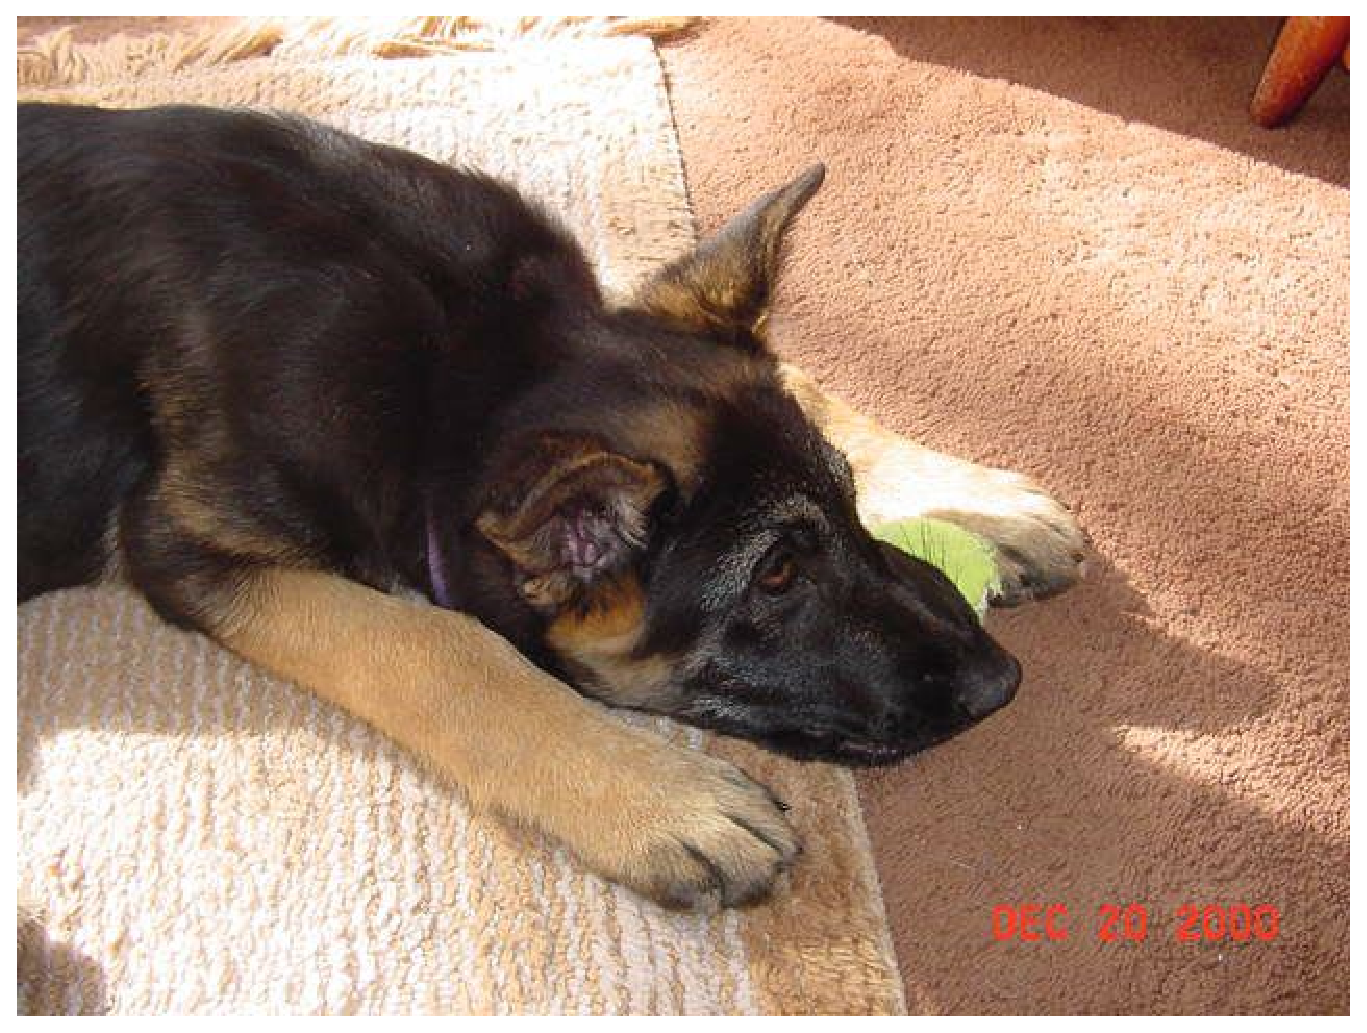
\includegraphics[height=1.5in,width=2.0in]{pup-on-rug}
\caption{An example of an imported eps file.}
\label{f:ex}
\end{figure}
\index{commands!environments!figure}%
You can see the commands that generated this
figure in the source file. Look for the line
\cn{begin\{figure\}[htb] \% Imported eps example. }

The command that imports the file is \cn{includegraphics}, and it also 
controls its size (\texttt{height} and \texttt{width}), and 
can rotate the figure (\texttt{angle}).

Figures can also be drawn by using \LaTeX{} commands. 
Figure \ref{f:circuit} is an example 
(taken from \cite{gms:tlc}).

\begin{figure}[htb] % Picture example.
\begin{center}
   \setlength{\unitlength}{4mm}
   \begin{picture}(12,10)(-2,0)
      \linethickness{0.4pt}
      \qbezier(2.00,6.00)(7.00,6.00)(9.00,3.00)
      \qbezier(2.00,0.00)(7.00,0.00)(9.00,3.00)
      \qbezier(2.00,6.00)(4.00,3.00)(2.00,0.00)
      \qbezier(1.00,6.00)(3.00,3.00)(1.00,0.00)
      \put(9.75,3.00){\circle{1.50}}
      \put(10.50,3.00){\line(1,0){1.50}}
      \put(0.00,5.00){\line(1,0){1.50}}
      \put(0.00,1.00){\line(1,0){1.50}}
   \end{picture}
\caption{An example of a picture}
\label{f:circuit}
\end{center}
\end{figure}
\index{picture}%

The commands that generated this
picture are in the source file following the line
\cn{begin\{figure\}[htb] \% Picture example.  }

The commands used have rather obvious meanings. In particular, 
the command \cn{qbezier} 
\index{commands!qbezier@\cn{qbezier}}%
draws a quadratic Bezier curve, 
defined by its two ending points, and a third point (whose 
coordinates are in the middle) that is used as control point. 
Figure \ref{f:qb} illustrates the effect of the control point:

%\begin{figure}[htb] % Bezier curves example.
\begin{figure}[h] % Bezier curves example.
\begin{center}
   \setlength{\unitlength}{.8mm}
   \begin{picture}(55,55)(-15,0)
      \linethickness{1pt}
      \qbezier(0,0)(-10,30)(50,30)
      \qbezier(0,0)(20,50)(50,30)
      \thinlines
      \put(0,0){\line(-1,3){10}}
      \put(50,30){\line(-1,0){60}}
      \put(0,0){\line(2,5){20}}
      \put(50,30){\line(-3,2){30}}
      \put(0,0){\circle*{1}}
      \put(0,-1){\makebox(0,0)[t]{$A_{0,0}$}}
      \put(-10,30){\circle*{1}}
      \put(-10,31){\makebox(0,0)[b]{$B_{10,30}$}}
      \put(50,30){\circle*{1}}
      \put(58,29){\makebox(0,0)[b]{$C_{50,30}$}}
      \put(20,50){\circle*{1}}
      \put(20,51){\makebox(0,0)[b]{$D_{20,50}$}}
   \end{picture}
\caption{Bezier curves}
\label{f:qb}
\end{center}
\end{figure}
\index{Bezier curves}%


This figure has been generated with the following commands:
\begin{verbatim}
\begin{figure}[htb] % Bezier curves example.
\begin{center}
   \setlength{\unitlength}{.8mm}
   \begin{picture}(55,55)(-15,0)
      \linethickness{1pt}
      \qbezier(0,0)(-10,30)(50,30)
      \qbezier(0,0)(20,50)(50,30)
      \thinlines
      \put(0,0){\line(-1,3){10}}
      \put(50,30){\line(-1,0){60}}
      \put(0,0){\line(2,5){20}}
      \put(50,30){\line(-3,2){30}}
      \put(0,0){\circle*{1}}
      \put(0,-1){\makebox(0,0)[t]{$A_{0,0}$}}
      \put(-10,30){\circle*{1}}
      \put(-10,31){\makebox(0,0)[b]{$B_{10,30}$}}
      \put(50,30){\circle*{1}}
      \put(58,29){\makebox(0,0)[b]{$C_{50,30}$}}
      \put(20,50){\circle*{1}}
      \put(20,51){\makebox(0,0)[b]{$D_{20,50}$}}
   \end{picture}
\caption{Bezier curves}
\label{f:qb}
\end{center}
\end{figure}
\end{verbatim}



%\chapter{An Example of Mathematical Writing}
\index{An Example of Mathematical Writing%
@\emph{An Example of Mathematical Writing}}%

\section{Generalized Fatou's Lemma}
\index{Generalized Fatou's Lemma%
@\emph{Generalized Fatou's Lemma}}%

Here we show an application of the following lemma:

\begin{lem}[Generalized Fatou's Lemma] \label{l:fatou}

Let $A$ be a Dedekind ring and $F$ a rational series 
in $A[[X]]$, i.e., $F = p/q$ for some 
$p, q \in A[X]$. Then there exist two polynomials 
$P, Q \in A[X]$ such that $F = P/Q$, 
where $P$ and $Q$ are relatively prime and 
$Q(0) = 1$.

\end{lem}

\proof
See \cite{bertin:psn}, p.~15, theorem~1.3.
\endproof

\begin{thm} \label{l:req}
Let $\{c_n\}_{n=-\infty}^{\infty}$ a set of 
elements from $K$ such that $c_n \in k'$ for every 
$n \geq n_0$, and verifying the following recurrence 
relation of order M:
\begin{equation}
c_n\ =\ r_1\,c_{n-1} + r_2\,c_{n-2} + \dots + r_M\,c_{n-M}
\end{equation}
for every $n \in \mathbb Z$, where $r_1,r_2,\dots,r_M$ are in 
$K$, $r_M \neq 0$. 
Then:

\item{(i)} The coefficients $r_1,r_2,\dots,r_M$ are in 
$k'$, and for every $n \in \mathbb Z$, $c_n \in k'$.

\item{(ii)} If $c_n \in \mathcal O_{k',v}$ 
for every $n \geq n_0$, then the coefficients 
$r_1,r_2,\dots,r_M$ are all in 
$\mathcal O_{k',v}$.

\end{thm}


\proof 

\item{(i)} Let $C_n$ and $R$ be the matrices:

\begin{equation}
C_n\ =
\ \left(
\begin{array}{llll}
              c_n & c_{n+1} & \hdots & c_{n+M-1} \\
              c_{n+1} & c_{n+2} & \hdots  & c_{n+M} \\
              \vdots & \vdots & \ddots & \vdots \\
              c_{n+M-1} & c_{n+M} & \hdots & c_{n+2M-2}
\end{array}
\right)
\end{equation}
and
\begin{equation}
R\ =
\ \left(
\begin{array}{lllll}
              0 & 1 & 0 & \hdots & 0 \\
              0 & 0 & 1 & \hdots & 0 \\
             \vdots & \vdots & \vdots & \ddots & \vdots \\
              0 & 0 & 0 & \hdots & 1 \\
              r_M & r_{M-1} & r_{M-2} & \hdots & r_1 
\end{array}
\right)
\end{equation} 

We have that $C_{n+1} = R\,C_n$. Since the recurrence 
relation is of order M, $C_n$ is non singular. 
On the other hand, $R = C_{n+1}\,C_{n}^{-1}$. Since the 
elements of $C_n$ are in $k'$ for $n \geq n_0$, the entries 
of $R$, and those of $R^{-1}$, will be in $k'$. Since 
$C_{n-1} = R^{-1}\,C_n$, we get that the entries of 
$C_n$ will be in $k'$ also for $n < n_0$. 

\item{(ii)} For each $t \geq n_0$ define the formal 
power series 

\begin{equation}
F_t(X)\ =\ \sum_{n=0}^{\infty} c_{t+n}\,X^n
\end{equation}
which is in $\mathcal O_{k',v}[[X]]$. 
We have $F_t(X) = p_t(X)/q(X)$, 
where $p_t(X),q(X) \in k'[X]$ are the following:
\begin{equation}
p_t(X)\ =\ \sum_{j=0}^{M-1} \Bigl( c_{t+j} - 
                    \sum_{i=1}^{j} r_i\,c_{t+j-i} \Bigr)\,X^j
\end{equation}
\begin{equation}
q(X)\ =\ 1 - r_1\,X - r_2\,X^2 - \dots - r_M\,X^M
\end{equation}
This can be checked by multiplying $F_t(X)$ by $q_t(X)$ 
and using the recurrence relation, which gives 
$F_t(X)\,q(X) = p_t(X)$ (see \cite{poorten:sp}). 

Now we will prove that $p_t(X)$ and $q(X)$ are relatively 
prime. To do so, we will see that they cannot have any 
common root (in $\overline {k'}$). In fact, assume 
that $\alpha$ is a common root of $p_{t_0}(X)$ and $q(X)$ 
for some $t_0 \geq n_0$, i.e.: 
$p_{t_0}(\alpha) = q(\alpha) = 0$. 
Since $q(0)=1$, then $\alpha \neq 0$. Now we have:
\begin{equation}
X\,F_{t_0+1}(X) = F_{t_0}(X) - c_{t_0}
\end{equation}
so:
\begin{multline}
X\,p_{t_0+1}(X) = X\,q(X)\,F_{t_0+1}(X) \\
= q(X)\,(F_{t_0}(X) - c_{t_0}) = p_{t_0}(X) - c_{t_0}\,q(X)
\end{multline}
Hence $p_{t_0+1}(\alpha) = 0$, which means that $\alpha$ is 
also a root of $p_{t_0+1}(X)$. By induction we get that 
$p_t(\alpha) = 0$ for every $t \geq t_0$. Grouping the 
terms of $p_t(X)$ with respect to $c_t,c_{t+1},\dots,c_{t+M-1}$, 
we get:
\begin{equation}
p_t(X) = \sum_{j=0}^{M-1} a_j(X)\,c_{t+j}
\end{equation}
where 
\begin{equation}
a_j(X) = X^j\,\Bigl( 1 - \sum_{i=1}^{M-j-1} r_i\,X^i \Bigr)
\end{equation}
Note that $a_0(X),a_1(X),\dots,a_{M-1}(X)$ do not depend on t. 
On the other hand $p_t(\alpha)=0$ implies
\begin{equation}
\label{e:coldep}
\sum_{j=0}^{M-1} a_j(\alpha)\,c_{t+j} = 0
\end{equation}
for every $t \geq t_0$. Note that $a_{M-1}(\alpha)=\alpha^{M-1}
\neq 0$, so $a_0(\alpha),a_1(\alpha),\dots,a_{M-1}(\alpha)$ 
are not all zero, and (\ref{e:coldep}) means that the columns 
of the matrix $C_{t_0}$ are linearly dependent, so 
$\det C_{t_0}=0$, which contradicts the fact that $C_{t_0}$ 
is non singular. Hence, the hypothesis that $p_t(X)$ and 
$q(X)$ have a common root has to be false. This proves that 
$p_t(X)$ and $q(X)$ are relatively prime. 

By (generalized Fatou's) lemma~\ref{l:fatou}, 
and taking into account that 
$\mathcal O_{k',v}$ is a Dedekind ring, 
we get that there exist two relatively prime 
polynomials $P_t(X)$ and $Q_t(X)$ in 
$\mathcal O_{k',v}[X]$ such that 
$F_t(X) = P_t(X)/Q_t(X)$ and $Q_t(0)=1$. Hence: 
$p_t(X)\,Q_t(X) = q(X)\,P_t(X)$. By unique factorization 
of polynomials in $k'[X]$, there is a $u \in k'$ such that 
$P_t(X) = u\,p_t(X)$ and $Q_t(X) = u\,q_t(X)$. Since 
$Q_t(0)=q(0)=1$, we get that $u=1$, so 
$P_t(X) = p_t(X)$ and $Q_t(X) = q(X)$. 
Hence, the coefficients of $q(X)$ are in 
$\mathcal O_{k',v}$. 

\endproof


\section{Other Examples of Mathematical Writing}

\subsection{An Example of a Commutative Diagram}
\index{An Example of a Commutative Diagram%
@{An Example of a Commutative Diagram}}%

The following is an example of a commutative diagram.
\index{commutative diagram}%
It requires the \texttt{amscd} package.
\index{amscd package@{\texttt{amscd} package}}

\begin{equation*}
\newcommand{\End}{\operatorname{End}}
\begin{CD}
S^{{\mathcal{W}}_\Lambda}\otimes T   @>j>>   T\\
@VVV                                    @VV{\End P}V\\
(S\otimes T)/I                  @=      (Z\otimes T)/J
\end{CD}
\end{equation*}

That diagram has been made with the following commands:

\begin{verbatim}
\newcommand{\End}{\operatorname{End}}
\begin{CD}
S^{{\mathcal{W}}_\Lambda}\otimes T   @>j>>   T\\
@VVV                                    @VV{\End P}V\\
(S\otimes T)/I                  @=      (Z\otimes T)/J
\end{CD}
\end{verbatim}

\subsection{Using AMS Fonts}
\index{Using AMS Fonts@{Using AMS Fonts}}

To use AMS fonts it is necessary to choose from an assortment 
of \LaTeX{} packages. For instance the command 
\cn{usepackage\{amsfonts\}} calls in the \emph{amsfonts} package, 
which provides blackboard bold letters (e.g. $\mathbb{R}$) and 
some math symbols. A superset of that package is 
\emph{amssymb}. Other packages are \emph{eufrak} 
for Frankfurt letters (e.g. $\mathfrak{R}$)
and \emph{eucal} for Euler script 
(e.g. $\mathcal{R}$). 
Consult the \LaTeX{} documentation about this subject 
for additional information.



%%%%%%%%%%%%%%%%%%%%%%%%%%%%%%%%%%%%%%%%%%%%%%%%%%%%%%%%%%%%%%%%%%%%%%
% Appendix/Appendices                                                %
%%%%%%%%%%%%%%%%%%%%%%%%%%%%%%%%%%%%%%%%%%%%%%%%%%%%%%%%%%%%%%%%%%%%%%
%
% If you have only one appendix, use the command \appendix instead
% of \appendices.
%
\appendices
\index{Appendices@\emph{Appendices}}%

\chapter{Lerma's Appendix}
\index{Appendix!Lerma's Appendix@\emph{Lerma's Appendix}}%
The source \LaTeX{} file for this document is no longer quoted in
its entirety in the output document. A \LaTeX{} file can 
include its own source by using the command
\cn{verbatiminput\{\cn{jobname}\}}.



%%%%%%%%%%%%%%%%%%%%%%%%%%%%%%%%%%%%%%%%%%
\chapter{My Appendix \#2}
\index{Appendix!My Appendix \#2@\emph{My Appendix \#2}}%
\section{The First Section}
This is the first section.
This is the second appendix.

\section{The Second Section}
This is the second section of the second appendix.

\subsection{The First Subsection of the Second Section}
This is the first subsection of the second section of the second appendix.

\subsection{The Second Subsection of the Second Section}
This is the second subsection of the second section of the second appendix.

\subsubsection{The First Subsubsection of the Second Subsection of
		the Second Section}
This is the first subsubsection of the second subsection of the
second section of the second appendix.

\subsubsection{The Second Subsubsection of the Second Subsection
		of the Second Section}
This is the second subsubsection of the second subsection of the
second section of the second appendix.


%%%%%%%%%%%%%%%%%%%%%%%%%%%%%%%%%%%%%%%%%%
\chapter{My Appendix \#3}
\index{Appendix!My Appendix \#3@\emph{My Appendix \#3}}%

\section{The First Section}
This is the first section.
This is the third appendix.

\section{The Second Section}
This is the second section of the third appendix.





%%%%%%%%%%%%%%%%%%%%%%%%%%%%%%%%%%%%%%%%%%%%%%%%%%%%%%%%%%%%%%%%%%%%%%
% Generate the bibliography.					     %
%%%%%%%%%%%%%%%%%%%%%%%%%%%%%%%%%%%%%%%%%%%%%%%%%%%%%%%%%%%%%%%%%%%%%%
%								     %
% NOTE: For master's theses and reports, NOTHING is permitted to     %
%	come between the bibliography and the vita. The command      %
%	to generate the index (if used) MUST be moved to before      %
%	this section.						     %
%								     %
\nocite{*}      % This command causes all items in the 		     %
                % bibliographic database to be added to 	     %
                % the bibliography, even if they are not 	     %
                % explicitly cited in the text. 		     %
		%						     %


%%%%%%%%%%%%%%%%%%%%%%%%%%%%%%%%%%%%%%%%%%%%%%%%%%%%%%%%%%%%%%%%%%%%%%
% Generate the index.						     %
%%%%%%%%%%%%%%%%%%%%%%%%%%%%%%%%%%%%%%%%%%%%%%%%%%%%%%%%%%%%%%%%%%%%%%
%								     %
% NOTE: For master's theses and reports, NOTHING is permitted to     %
%	come between the bibliography and the vita. This section     %
%	to generate the index (if used) MUST be moved to before      %
%	the bibliography section.				     %
%								     %
%\printindex%    % Include the index here. Comment out this line      %
%		% with a percent sign if you do not want an index.   %
%%%%%%%%%%%%%%%%%%%%%%%%%%%%%%%%%%%%%%%%%%%%%%%%%%%%%%%%%%%%%%%%%%%%%%


\bibliographystyle{plain}  % Here the bibliography 		     %
\bibliography{thesis}        % is inserted.			     %
\index{Bibliography@\emph{Bibliography}}%			     %
%%%%%%%%%%%%%%%%%%%%%%%%%%%%%%%%%%%%%%%%%%%%%%%%%%%%%%%%%%%%%%%%%%%%%%

%%%%%%%%%%%%%%%%%%%%%%%%%%%%%%%%%%%%%%%%%%%%%%%%%%%%%%%%%%%%%%%%%%%%%%
% Vita page.							     %
%%%%%%%%%%%%%%%%%%%%%%%%%%%%%%%%%%%%%%%%%%%%%%%%%%%%%%%%%%%%%%%%%%%%%%

\end{document}
